\documentclass{article}
\usepackage[utf8]{inputenc}
\usepackage{algorithm}
\usepackage[noend]{algpseudocode}

\usepackage[magyar,greek,english,german]{babel}
\usepackage{amsmath,amsfonts,amssymb,amsthm}
\usepackage[hyphens]{url}
\usepackage{hyphenat}
\usepackage{graphicx}
\usepackage{listings}
\usepackage{mathtools}
\usepackage[dvipsnames]{xcolor}
\usepackage{longtable}
\setlength{\fboxsep}{0pt} % for \colorbox

\floatname{algorithm}{Algoritmus}
\algrenewcommand\algorithmicwhile{\textbf{amíg}}
\algrenewcommand\algorithmicdo{\textbf{végezd el}}
\algrenewcommand\algorithmicend{\textbf{vége}}
\algrenewcommand\algorithmicif{\textbf{ha}}
\algrenewcommand\algorithmicthen{\textbf{akkor}}
\algrenewcommand\algorithmicelse{\textbf{különben}}
\algrenewcommand\algorithmicprocedure{\textbf{eljárás}}
\algrenewcommand\algorithmicfor{\textbf{ciklus}}
\algrenewtext{EndWhile}{\algorithmicwhile\ \algorithmicend}

\lstset{
  basicstyle=\footnotesize\ttfamily,
  mathescape,
  morekeywords={*,text1,text2,lookup1,lookup2,find1,find2,getrefs,extend,minunique1,latintext1,latintext2},
  keywordstyle=\color{blue},
  breaklines=true,
  breakatwhitespace=true
}

\tolerance10000
\newcommand\gr{\selectlanguage{greek}\frenchspacing}
\newcommand\hu{\selectlanguage{magyar}\frenchspacing}
\newcommand\en{\selectlanguage{english}\frenchspacing}
\newcommand\de{\selectlanguage{german}\frenchspacing}

\newcommand\Luke{{\color{Lavender}\bullet}\mathllap{\color{Lavender}\circ}}
\newcommand\Paul{{\color{YellowGreen}\bullet}\mathllap{\color{YellowGreen}\circ}}
\newcommand\Unknown{{\color{Orchid}\bullet}\mathllap{\color{Orchid}\circ}}
\newcommand\Matthew{{\color{Red}\bullet}\mathllap{\color{Red}\circ}}
\newcommand\Mark{{\color{Cyan}\bullet}\mathllap{\color{Cyan}\circ}}
\newcommand\John{{\color{GreenYellow}\bullet}\mathllap{\color{GreenYellow}\circ}}
\newcommand\Peter{{\color{NavyBlue}\bullet}\mathllap{\color{NavyBlue}\circ}}

\newtheorem{theorem}{Tétel}

\begin{document}

\hu
\title{Ószövetségi idézetek \\automatikus azonosítása\\ az Újszövetségben\\
\textsc{(félkész vázlat)}}
\author{Kovács Zoltán\\ \de Private Pädagogische Hochschule der Diözese Linz\\
Salesianumweg 3, 4020 Linz,\hu\ Ausztria}
\maketitle

\section{Bevezetés}
Keresztény hitünk egyik fontos eleme a Biblia belső hivatkozásainak rendszere.
Az evangéliumok híradása szerint Jézus számos alkalommal idéz az Ószövetségből, de
a többi újszövetségi szerzőnél is gyakran találunk ószövetségi idézeteket.

Jézus saját misszióját az ószövetségi előzménybe helyezi be:
\begin{itemize}
\item \textit{Ne gondoljátok, hogy azért jöttem, hogy érvénytelenné tegyem a törvényt
vagy a próféták tanítását. Nem azért jöttem, hogy érvénytelenné tegyem, hanem hogy betöltsem azokat.
Mert bizony mondom néktek, hogy amíg az ég és a föld el nem múlik, egy ióta vagy egy vessző
sem vész el a törvényből, míg minden be nem teljesedik.} (Mt 5:17-18)\footnote{Ahol külön
nem jelöltük, ott a bibliai szövegeket az \cite{UFO} fordításból vettük.}
\item \textit{Mert ha hinnétek Mózesnek, hinnétek nekem: mert énrólam írt ő.} (Jn 5:46)
\item \textit{$\ldots$az Emberfián beteljesedik az, amit a próféták megírtak.} (Lk 18:31)
\item \textit{$\ldots$be kell teljesednie mindannak, ami meg van írva rólam a Mózes törvényében,
a próféták könyvében és a zsoltárokban.} (Lk 24:44)
\end{itemize}
Jézus többször hivatkozik a \textit{törvényre} és a \textit{prófétákra} (Mt 7:12, Mt 22:40), valamint
a \textit{zsoltárokra} (Lk 24:44, Mt 26:30, Mk 14:26). Ezekre a szövegekre néhol egészen hosszan utal
(mint pl. a Mt 21:42-ben), máshol csak pár szóban (mint pl. a Lk 22,37-ben).

Az időrendet követve Jézus halála és feltámadása után bizonyos újszövetségi szerzőknél hosszú gondolatmeneteket olvasunk,
melyek ószövetségi alapokon állnak. Az egyik kiemelkedő szerző Pál apostol, aki a Római levélben
mintegy 60 ószövetségi szakaszt idéz, többnyire betű szerint. Ez egybevág azzal, ahogyan
Az apostolok cselekedeteiben megismerjük őt, amint -- például -- Thesszalonikában a zsidók zsinagógájában
vitázik:
\begin{quote}
\textit{Pál pedig szokása szerint bement hozzájuk, és három szombaton is vitába
szállt velük az Írások alapján. Megmagyarázta és bizonyította nekik, hogy
Krisztusnak szenvednie kellett, és fel kellett támadnia a halálból.} (ApCsel 17:2-3)
\end{quote}
Az Apostolok cselekedetei feljegyzéseinek alapján azonban nemcsak Pál, hanem munkatársa,
Apollós is \textit{a nyilvánosság előtt bizonyította az Írások alapján, hogy Jézus a Krisztus}
(ApCsel 18:28). 

Az Ószövetség használata tehát a keresztény érvelésben aligha elkerülhető. De milyen módon lehet
az Ószövetséget korrekt módon alkalmazni? Még a Sátánról is olvassuk, hogy Jézus megkísértése
során egy zsoltárt idéz: 
\begin{quote}
\textit{``Ha Isten Fia vagy, vesd le magadat innen, mert meg van írva:
Angyalainak megparancsolta, hogy őrizzenek téged; 
és tenyerükön hordoznak, hogy meg ne üsd lábadat a kőben.''
Jézus így válaszolt neki: ``Megmondatott: Ne kísértsd az Urat, a te Istenedet.''} (Lk 4:9-12)
\end{quote}
A Sátán a 91. zsoltár 11-12. verseit idézi, míg Jézus az 5Móz 6:16-ot. S itt megjegyezzük,
hogy Jézus a Sátán másik kísértő gondolatára (l. Mt 4:1-9 ill. Lk 4:1-13) is ószövetségi szakaszokkal
(ti. az 5Móz 8:3-mal, valamint az 5Móz 6:13-mal és az 5Móz 10:20-szal) felel.

A modern bibliaolvasó emberben azonban kíváncsiság támadhat, hogy vajon az újszövetségi idézetek
valóban az Ószövetségen alapulnak-e. Vajon minden esetben beazonosítható, hogy a törvény mely
részéből ill. melyik prófétától, esetleg melyik zsoltárból származik a kérdéses idézet?
Továbbá, az idézet pontos-e? Valamint: Nem lehetséges-e, hogy bizonyos újszövetségi szerzők az egyes
idézeteket a saját érvelésük előnyére átalakították, arról nem is beszélve, hogy változatás
nélkül átvéve gondolatokat a saját kontextusukba helyezve esetleg új értelmet adtak a szövegnek?

Ezekre a kérdésekre válaszolni olyannyira nem egyszerű, hogy a témának óriási teológiai irodalma
van, amelyben egészen apró kérdések, akár konkrét igehelyek pontosabb értelmezése is
hosszú tanulmányok központi gondolata lehet. Ebben az írásban is csak néhány konkrét kérdéssel
foglalkozunk, főként olyanokkal, amelyek számítógépes vizsgálatokkal megközelíthetőek.

\subsection{Szövegkritikai háttér}

Amikor Bibliáról beszélünk, nehéz pontosan megmondanunk, hogy mire is gondolunk. Legtöbbször
egy bibliafordítást tartunk a kezünkben, ami egy vagy több korábbi dokumentumon alapul,
melyek jórészt még korábbi dokumentumoknak a másolatai, gyakran másolási hibákat vagy
több lehetséges szövegvariációt magukon hordozva. Ezeket a korábbi dokumentumokat
(melyeket kézzel írtak) kéziratoknak nevezzük.

Számos kéziratnak létezik számítógépes feldolgozása, amelyek a szöveget
digitálisan kódolt formában tartalmazzák, esetlegesen az egyes szövegvariációkat
is megtartva. Amikor tehát arra vagyunk kíváncsiak, hogy Jézus valóban az 5Móz 6:16-ot idézi-e
a Lk 4,12-ben, akkor legalább a következő kérdéseket fel kell, hogy tegyük:
\begin{enumerate}
\item Milyen nyelven beszélt Jézus és milyen nyelven jegyezték le? -- Ismereteink szerint
Jézus arámi nyelven beszélt, de Lukács (ill. Máté, Márk és János) görögül jegyezték le a szavait.
\item Milyen nyelven íródott az Ószövetség? -- Az Ószövetség héber nyelven íródott,
de az I. században, vagyis az első keresztények számára rendelkezésre állt annak
görög nyelvű fordítása, amelynek kisebb-nagyobb részleteit későbbre datálható kéziratokból
ismerjük. Így rendelkezésünkre áll többek között
\begin{itemize}
\item a Sínai-félszigeti kódex,
a Codex Sinaiticus, hivatalos számozással $\boldsymbol{\aleph}$ vagy \textbf{01}, ami 330 és 360 között keletkezhetett,
\item a Vatikáni kódex, a Codex Vaticanus, hivatalos számozással \textbf{B} vagy \textbf{03} (a mai ismereteink szerint 300 és 325 között keletkezett),
\item az Alexandriai kódex, a Codex Alexandrinus, melynek keletkezése 400 és 440 közé tehető,
hivatalos kódja \textbf{A} vagy \textbf{02},
\end{itemize}
melyek a ma ismert Bibliának nagy részét tartalmazzák, kisebb-nagyobb különbségekkel.
\end{enumerate}
Habár Jézus és közvetlen tanítványai között a kommunikáció valószínűleg arámi nyelven zajlott,
az akkori események feljegyzésére görögül került sor. A héber nyelvű Ószövetség
görög fordítása Kr. e. 300 körül készült az egyiptomi Alexandriában, II. Ptolemaiosz fáraó idején.
Erre a fordításra \textit{Septuaginta} néven hivatkozunk.
A latin nyelvű ``septuaginta'' szó 70-et jelent, és arra utal, hogy a fordítást hetvenkét zsidó bölcs
készítette, akik tizenkét zsidó törzs tagjai voltak: minden törzset hatan képviseltek a fordítás elkészítésekor.
Jogos azonban a kérdés, hogy ez a fordítás hűen tükrözi-e az eredeti tartalmat. A kétkedők
gyorsan találhatnak olyan példát, ahol a görög fordítás más árnyalatot, netalántán valamelyest
új tartalmat is hordoz.

\subsubsection{A maszoréta szöveg és a Holt tengeri tekercsek}

Hiába tehát a legendás háttértörténet, sokak számára a Septuaginta csak másodlagos forrása
Isten Igéjének. Fontos tény továbbá, hogy a Septuaginta nem ad vissza olyan, csak a héber szövegben feltűnő
jellegzetességeket, mint pl. a 119. zsoltár 22 versszaka, amelyekben a 8-ból minden egyes vers
ugyanazzal a héber betűvel kezdődik. Az ilyen jellegzetességeket nem csupán a Septuaginta, hanem lényegében
egyetlen más fordítás sem őrzi, így joggal kijelenthetjük, hogy a héber szöveg
ebben a tekintetben is egyedülálló.

Sok bibliafordítás (főként a protestáns fordítások) az Ószövetség szövegénél egyértelműen a héber szöveget
részesíti előnyben. Még akkor is, ha a legrégebbi teljes héber nyelvű Ószövetség,
az Aleppói kódex jóval fiatalabb, mint a legrégebbi teljes görög nyelvű Ószövetség-fordítás:
a héber szöveg 10. századi, míg a görög a 4. századból való. Fontos érv azonban a héber szöveg
használata mellett, hogy a szöveget nemzedékeken át továbbadó maszoréták igen szakszerűen és pontosan
másolták a szöveget, és a korábbi tekercseket szántszándékkal mindig eltemették. A maszoréták
gondos munkája mellett szól az az érv is, hogy az 1. századból származó héber nyelvű Holt tengeri tekercsek tartalma
kevés eltérést mutat az Aleppói kódextől. Mindazonáltal meg kell jegyeznünk, hogy
az eltérések nagyságának megítélése az irodalomban elég szubjektív.

Így pl. Burrows szerint \cite[304. o.]{Burrows} bizonyos ószövetségi könyveknél kevés különbség van 1000 év távlatában,
más könyveknél azonban a különbség elég jelentős. Burrows itt Geisler és Nix széles körben
elterjedt és gyakran említett eredményét idézi, mely szerint:
\begin{quote}
Az Ézsaiás 53-ban 166 \textit{szó}
található, melyekben 17 \textit{betű}nyi eltérés van a két szöveg között.
Ezek közül 10 csupán helyesírási variáns, melyeknek ugyanaz a jelentése.
4 további betű apró stilisztikai különbséget takar (pl. kötőszavakat).
A maradék 3 betű egy betoldott szóban, a 11. versben található, ennek jelentése: ``fény'',
és ez sem változtatja meg a szöveg értelmét jelentősen. \cite[263. o.]{GeislerNix}
\end{quote}
Nemrégiben azonban Jeff Benner maga is nekilátott, hogy ellenőrizze ezeket az információkat
\cite{Benner}. Weboldalán részletesen közzéadja, hogy mire jutott:
\begin{quote}Az 53. fejezet 1. versével kezdve hamar megtaláljuk az első 17 betűt,
melyben eltér az Ézsaiás-tekercs és a maszoréta szöveg. Csak az első 3 versben --
melyekben összesen 23 szó szerepel a maszoréta szövegben ill. 24 a nagy Ézsaiás-tekercsben --
19 betűt találtam, amelyben a két szöveg különbözik.
\end{quote}
Bennerről egyáltalán nem mondható el, hogy ne lelkesedne az ószövetségi iratokért,
így eredményének ellenőrzése nélkül is hitelt adhatunk számításainak; munkáját azonban
részletesen dokumentálta. A fenti ellentmondás
feloldásaképpen nyilvánvalóan konkrétan ellenőrizni kéne a két szöveget \textit{gépi algoritmussal},
olyan módon, hogy bárki számára reprodukálható legyen az ellenőrzés, akár az utolsó
betűkig. Ehhez elsődleges,
hogy mind a szövegek, mind a számítógépes program ill. annak működése nyilvánosan
hozzáférhető legyen.

Más könyveket vizsgálva Fagan és Beck is kiemelik, hogy 
a Holt-tengeri tekercsek ill. az Aleppói kódex bizonyos könyvei között egészen komoly különbségek is
kimutathatóak \cite{FaganBeck}: ``Egy 1996-os archeológiai kötet szerint pl. a 2Mózes és
Sámuel könyvei olyannyira eltérnek egymástól 1000 év távlatában, hogy
arra a következtetésre kell jutni: a krisztusi idők előtt az Ószövetség
szövege egyáltalán nem szilárdult még meg.''

Ennél is messzebb megy Joseph Gleason, aki arra jut, hogy a maszoréta szövegből lényeges
elemek hiányoznak, és emögött akár szándékos mulasztás is állhat \cite{Gleason}.
Gleason több fontos újszövetségi idézetet is felsorol Jézussal kapcsolatosan, amelyek ószövetségi
referenciáiból valamilyen
részlet nyilvánvalóan hiányzik a maszoréta szövegben, holott az információ a Septuagintában
egyértelműen jelen van. Többek között a Zsid 10:5-öt, a Mt 1:23-at, a Zsid 1:6-ot, a Lk 4:18-at
vagy a Mt 12:21-et említi, és ezek a példák az olvasó számára is könnyen leellenőrizhetőek.

A maszoréták védelmében azonban meg kell jegyeznünk, hogy előfordulhat,
hogy ezek a különbségek már az első századokban bekerültek a héber szövegbe, és
az írnokok -- hiába igyekeztek hiba nélkül másolni -- már egy hiányos vagy pontatlan
változatot másoltak tovább. S még ha a maszoréta szövegről kiderül, hogy nem ér fel
a Septuaginta pontosságával, akkor is adható lenne egy numerikus érték, hogy összességében mekkora
eltéréssel kell számolnunk. Vélhetően feltűnően kicsivel. Tehát a maszoréta szöveg
még esetleges tökéletlenségében is elegendően tökéletes ahhoz, hogy Isten üzenetét hordozza.

\subsubsection{A Septuaginta}

Talán a fenti problémák is hozzájárultak ahhoz, hogy
az elmúlt évtizedekben a kutatások egy komoly része a Septuaginta irányába fordult,
különösen a Sínai-félszigeti kódexszel a középpontban. Világossá vált, hogy
az újszövetségi szerzőkre a görög fordítás komoly hatást gyakorolt, sőt, mi több:
letagadhatatlan a betű szerinti egyezés igen hosszú görög ószövetségi és
újszövetségi szakaszok között. Hogy csak egy példát említsünk, a Zsid 2:6-8
egyértelműen a Septuaginta-szövegre utal, amely segítségével Jézusról azt vezeti le
a szerző, hogy nagyobb az angyaloknál -- ez a gondolat a héber eredetiből nehezen olvasható ki.

Az ortodox egyházakban valójában már a kezdetektől a Septuaginta-fordítás a mérvadó,
viszont a protestáns fordításokban továbbra is a maszoréta szöveg a meghatározó.
Ennek ellenére Robert Henry Pfeiffer (1892-1958) metodista teológus már 1948-ban azt állította, hogy
az újszövetségi idézetek 80\%-a a Septuagintán alapul \cite{Pfeiffer}. A téma mai aktualitását
mutatja, hogy
de Vries és Karrer egy nemrégiben írt könyvbevezetőben \cite[3. o.]{deVriesKarrer} arról számolnak be,
hogy a 2010-es években igen aktív Wuppertal projekt Septuaginta-adatbázisában 357 idézett ószövetségi igeverset
azonosítottak be,
melyek az Újszövetségben 449 helyen jelennek meg.

Könnyen lehet azonban pontatlan következtetésekre
jutnunk, amire többek között A. Perry \en\textit{Did the NT writers ``quote''
the Septuagint?}\hu\ írása \cite{Perry} is figyelmeztet. Így tehát az a kijelentés, hogy
az újszövetségi szerzők a Septuagintából idéztek (és nem a héber szövegből), már
abban is pontatlan lehet, hogy a Septuaginta mint olyan akár nem is létezik, mivel nem bizonyítható,
hogy a héber szöveg görög fordítását bárki is így nevezte volna a 2. század előtt (l.
\cite[32., 89. o.]{JobesSilva}). Perry arra jut, hogy Isten \textit{Szelleme} az, aki idéz, és nem a Septuagintát,
hanem a saját \textit{Szavát}, mely héberül és arámi nyelven lett kijelentve -- viszont a kommunikáció az újszövetségi szerzőkben
testet öltve görögül történik. Ez a vélemény teológiailag megalapozottnak tűnik,
gyakorlati szempontból azonban mégis nehezen megfogható. Árnyaltabb eredményre jut de Vries és Karrer \cite[16. o.]{deVriesKarrer},
akik szerint sok korai keresztény író tudatosan és gondosan idézte az Ószövetséget, habár nem mindegyikük
figyelt a pontos fogalmazásra.

A jelenlegi kutatások számos további kérdést vetnek fel, de ebben az írásban csak azokra szorítkozunk,
amelyeket számítógépes vizsgálattal meg lehet válaszolni. Egy számítógépes algoritmus számára
csak maga a nyers szöveg létezik: a mögöttes tartalom nem vizsgálható.
Nyilvánvaló, hogy gépi (azaz mechanikus,
a szöveg értelmét nagyrészt vagy teljes egészében figyelmen kívül hagyó) összehasonlítást csak
azonos nyelvű szövegeken érdemes végezni. Ez pedig csupán a (görög) Septuaginta és a görög nyelvű
Újszövetség között hajtható végre.

Az első gyakorlati probléma a fenti kódexek digitális elérhetősége:
\begin{itemize}
\item A Sínai-félszigeti kódex (a továbbiakban: \textbf{01})
elektronikus változata 2009 júliusa óta digitálisan is hozzáférhető a \url{www.codexsinaiticus.org} webcímen.
\item Másrészt a Vatikáni Kódex (a továbbiakban: \textbf{03}), mely
2015 óta a \url{https://digi.vatlib.it/view/MSS_Vat.gr.1209} címen elektronikusan is elérhető, nem férhető hozzá
digitalizált formában, vagyis csak a kódexlapok fényképei láthatók.
\item Az Alexandria kódexet a \url{www.bl.uk/manuscripts/Viewer.aspx?ref=royal_ms_1_d_viii_fs001r}
webcímen érhetjük el, de ott is csak fényképekkel.
\end{itemize}

Ezen kívül vannak további lehetőségeink is, ha a görög nyelvű szövegeket digitális formában kívánjuk
elemezni. Mi ebben a tanulmányban két szöveget használunk, amelyek a nagyközönség számára könnyen
elérhetőek a Sword \cite{Sword} elektronikus könyvtárban, de egyik sem azonos a fenti kéziratok szövegével:
\begin{itemize}
\item Az általunk LXX néven említett elektronikus szövegen egy 2008-ban készült Sword-modult fogunk érteni,
mely Alfred Rahlfs 1935-ös Septuaginta-szövegén alapul. Ez részint idejétmúlt, de ennél újabb, ingyenesen
elérhető digitális Sword-modul e tanulmány írásának kezdetén nem állt rendelkezésre.\footnote{
Az olvasó figyelmébe ajánljuk a \url{https://www.crosswire.org/sword/modules/ModDisp.jsp?modType=Bibles}
weboldalt, ahol időközben néhány újabb modul is elérhető. Ilyen pl. az ABPGRK, az \textit{Apostolic Bible Polyglot}
elektronikus kiadása.} Ez lesz tehát az ószövetségi
rész tanulmányozásához használt digitális adatforrásunk.
\item Az Újszövetséghez a Society of Biblical Literature's Greek New Testament
(SBLGNT) kiadást fogjuk használni.
\end{itemize}
Fontos kiemelni, hogy ezek az adatforrások egy-egy \textit{plauzibilis}, valószínűsíthető változatát adják
az eredeti görög szövegnek. Sok esetben teljesen vagy majdnem betű szerint egyeznek a \textbf{01} ill.
a \textbf{03} szövegével, így kiválóan alkalmasak gépi algoritmusok tesztelésére. Pontosabb következtetések
levonására azonban célszerű más elektronikus adatforrásokat is kipróbálni.

\subsection{Az összehasonlítás nehézsége}

Példaként vegyük a Lk 4:10-12-ben már említett két idézetet, melyet az SBLGNT-ben ebben a formában találunk:
\begin{quote}
\gr
γεγραπται γαρ οτι Τοις αγγελοις αυτου εντελειται περι σου του διαφυλαξαι σε, /
και οτι Επι χειρων αρουσιν σε μηποτε προσκοψης προς λιθον τον ποδα σου. /
και αποκριθεις ειπεν αυτω ο Ιησους οτι Ειρηται Ουκ εκπειρασεις κυριον τον θεον σου.
\end{quote}
\hu
A vershatárokat / (``osztás'') jellel jelöltük, habár tanulmányunkban a későbbiekben a modern
versfelosztásnak nem lesz jelentősége. A Biblia eredeti szövege sem fejezetekre,
sem versekre sincs felosztva, a fejezet- és verszámozás csupán a XIII. századtól (Stephen Langton munkája nyomán),
majd később a XVI. században (Santes Pagnino és Robertus Stephanus,
valamint az első bibliakiadók munkájaként) váltak általánossá és
elfogadottá.

Az LXX-ben a következő szöveget találjuk a Zsolt 91:11-12 helyen:
\begin{quote}
\gr
οτι τοις αγγελοις αυτου εντελειται περι σου του διαφυλαξαι σε εν πασαις ταις οδοις σου /
επι χειρων αρουσιν σε μηποτε προσκοψης προς λιθον τον ποδα σου
\end{quote}
\hu
Láthatóan itt még központozás sincs, és a kis- és nagybetűk között sincs
különbségtétel. Valójában a kéziratokban még a szóközöket sem
mindig jelzik, és az új sor sem mindig két szó közé esik.
Így célszerű feltételeznünk, hogy informatikai szempontból az egyes
bibliai könyvek egy, csupán a görög ábécé $24+1$ betűjéből álló nyers karakterláncot
képeznek, amelyekben sem szóköz, sem más karakter nem jelenik meg. (A $+1$ a szó végi
\gr ς\hu-nek felel meg.) Az egyszerűség
kedvéért a továbbiakban minden digitális formában lévő görög igeverset kisbetűvel
és központozás nélkül írunk, azonban a könnyebb áttekinthetőség kedvéért
a plauzibilis szóközt megtartjuk. Ez azonban nem jelenti azt, hogy a szóhatárokat
fixnek vesszük.

Miből gondolhatjuk, hogy a Sátán ill. Jézus idézetet mond? A Lk 4:10 elején a Sátán
a \gr γεγραπται γαρ\hu\ szófordulatot használja
(\textbf{hiszen meg van írva}\footnote{A félkövéren szedett szövegeket a Csia Lajos-féle
szó szerinti \cite{Csia} fordításból vettük.}), mire Jézus a Lk 4:12-ben az
\gr ειρηται\hu\ (\textbf{azt mondják})
kifejezéssel indítja válaszát.
Honnan tudhatjuk, hogy a Sátán a Zsoltárokból idéz? Vegyünk egy tipikus szót az SBLGNT-szövegből,
lehetőleg elegendően hosszút, és keressük meg, hogy megtalálható-e az LXX-ben. A BibleTime
c. programban (ez a Sword adatbázist használja) az egyes keresőszavak szó szerint indexelve
vannak, így az \gr αγγελοις\hu\ (\textsc{angyalok}\footnote{Kiskapitálisan
szedjük a nyers fordítással megadott magyar szövegeket.}) szóra 4 találatot kapunk: a 4Móz 24:12-t, az 1Sám 11:9-et,
az 1Kir 20:9-et, s végül a Zsolt 91:11-et. Ha a keresésbe felvesszük az \gr αυτου\hu\ (\textsc{övé}) szót is
(ez követi az \gr αγγελοις\hu\ szót az SBLGNT-ben), akkor a találat már egyértelmű.

Az LXX-beli találat beazonosítása után következhet az idézet pontosságának meghatározása.
\begin{center}
\begin{tabular}{p{5cm} p{5cm}}
LXX Zsolt 91:11-12 & SBLGNT Lk 4:10-11\\
\hline
{\hfill\break\gr οτι \textcolor{red}{τοις αγγελοις αυτου εντελειται περι σου του διαφυλαξαι σε}\hfill\break
εν πασαις ταις οδοις σου
\hfill\break \textcolor{blue}{επι χειρων αρουσιν σε μηποτε προσκοψης προς λιθον τον ποδα σου}} &
{\gr γεγραπται γαρ\hfill\break οτι \textcolor{red}{τοις αγγελοις αυτου εντελειται περι σου του διαφυλαξαι σε}\hfill\break
και οτι\hfill\break \textcolor{blue}{επι χειρων αρουσιν σε μηποτε προσκοψης προς λιθον τον ποδα σου}}
\end{tabular}
\end{center}
\hu\

Megfigyelhetjük, hogy az LXX-beli idézet középső (feketén hagyott) részét nem idézi a Sátán,
hanem helyette a \gr και οτι\hu\ (\textsc{és hogy}) szerkezettel jelzi a kihagyást. Fontos, hogy az indító \gr οτι\hu\ 
szócska a görög nyelv szabályai szerint nem része az idézetnek, de mivel ez a szó mindkét
szakaszban ott van a bevezetőben, egy gépi keresés során a találatot ezzel a szóval együtt kapnánk meg.

A Jézus által idézett válasz leghosszabb szavára rákeresve az LXX-ben egyetlen találatot kapunk,
és láthatóan az eredményül kapott szakasz betű szerint egyezik az SBLGNT-ben lévővel:
\begin{center}
\begin{tabular}{p{5cm} p{5cm}}
LXX 5Móz 6:16 & SBLGNT Lk 4:12\\
\hline
& {\gr και αποκριθεις ειπεν αυτω ο ιησους οτι ειρηται}\\
\gr \textcolor{red}{ουκ εκπειρασεις κυριον τον θεον σου} &
\gr \textcolor{red}{ουκ εκπειρασεις κυριον τον θεον σου} \\
\gr ον τροπον εξεπειρασασθε εν τω πειρασμω &
\end{tabular}
\end{center}
\hu
Ezek a találatok több fontos részletre világítanak rá:
\begin{itemize}
\item Egy idézett szöveg lehet \textit{egyedi}, vagyis csak egyetlen egyszer szerepel
az Ószövetségben. (Ezt az észrevételt később még pontosítani fogjuk, ugyanis néhány esetben
többször is megjelenik ugyanaz az idézett gondolat: néhol betű szerint, néhol kisebb variációval.)
Ez nem jelenti azt, hogy az idézet az Újszövetségben is feltétlenül csak egyszer szerepel, itt például
a Máté-féle párhuzamos helyen is megtaláljuk mindkét szakaszt. Feltűnhet azonban, hogy Máté a 91. zsoltár első szakaszát
két szóval rövidebben idézi, mint Lukács. 
\item Az idézet lehet \textit{pontos}, vagyis az ószövetségi idézett szöveg és az újszövetségi idézet megegyezhet
betű szerint teljes egészében.
\item Az idézet átnyúlhat modern beosztású igeverseken. Valójában a versbeosztás teljesen irreleváns,
és a későbbiekben egy ezen felül álló jelölésrendszert fogunk használni, ami egy digitális dokumentumhoz kapcsolt
modern beosztáshoz képest megadott \textit{relatív helyzetét} adja majd meg az idézett szövegnek ill. idézetnek.
Ha a modern beosztástól elvonatkoztatunk, akkor a digitális dokumentumban \textit{abszolút pozícióról} is beszélhetünk.
Ez a pozíció viszont mindig függ a digitális dokumentumtól.
\end{itemize}

A nehézségek akkor kezdődnek csak igazán, amikor egy digitális dokumentumból több variáció is létezik.
A \textbf{01}-ben a Lk 4,10 két variációt is említ: a \gr γεγραπται\hu\ (\textbf{meg van írva}) szó után az egyik
korrektor szerint megjelenik a \gr γαρ\hu\ (\textbf{hiszen}) szócska (\ref{Lk4:10-gar}. ábra). Ettől eltekintve a szöveg
teljes egészében megegyezik az SBLGNT szövegével -- attól az apróságtól eltekintve, hogy ebben a kódexben
(hasonlóan a többi ez időtájban készült irathoz) a görög szigma betűt a szó közepén és végén is
egységesen félholdszerűen írták, akárcsak a ma használatos c betűt.

\begin{figure}
\begin{center}
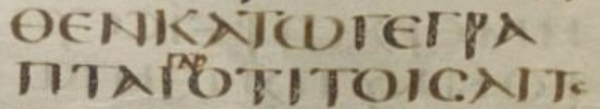
\includegraphics[width=0.5\textwidth]{../common/Lk4:10-gar}
\caption{Részlet a Lk 4:10-ből a Sínai-félszigeti kódexben}
\label{Lk4:10-gar}
\end{center}
\end{figure}

A \textbf{01}-ben megtalálható a 91. zsoltár is, de 90. sorszámon. Az idézett szöveghez kapcsolódó
tartalma teljes egészében megegyezik az LXX szövegével, azzal az egy különbséggel, hogy az
\gr επι\hu\ (\textsc{-ban/-ben}) elöljárószó elé egy \gr και\hu\ szócska is bekerül.

%οτι τοιϲ αγγελοιϲ αυτου εντελειται περι ϲου του διαφυλαξαι
%ϲε εν παϲαιϲ ταιϲ οδοιϲ ϲου 
%και επι χειρων αρουϲιν ϲε μηποτε προϲκοψηϲ προϲ λιθον τον ποδα ϲου

Az 5Móz 6:16 viszont nem található meg a \textbf{01}-ben. Az 5Móz-nek csupán néhány fejezete
maradt meg ebben a kéziratban, nevezetesen a 3., 4., 28., 29. és 30. fejezetek egy része
(és ezek is csak töredékesen, mert a kódexlapok megsérültek).

A \textbf{03} általában teljesebb, mint a \textbf{01}, azonban a kódex fényképeit nem
lehet gyorsan végigfutni, hanem részletesen ``át kell betűzni'' az oldalakat, ha egy
igeszakaszt meg akarunk találni. Esetünkben a Lk 4:10-11 az 1310. oldal jobb alsó sarkában
található (\ref{03-Lk4:10-11}. ábra), és egyetlen betűnyi eltérés van benne az SBLGNT-hez képest:
az \gr αρου{\hu c}ιν \hu\ (\textbf{hordozzanak}) szó végén lévő nű hiányzik. Ezt az apróságot nem könnyű észrevenni,
mert a szövegnek ez a része igen nehezen olvasható (az ábrán alulról a 3. sor elején található).

\begin{figure}
\begin{center}
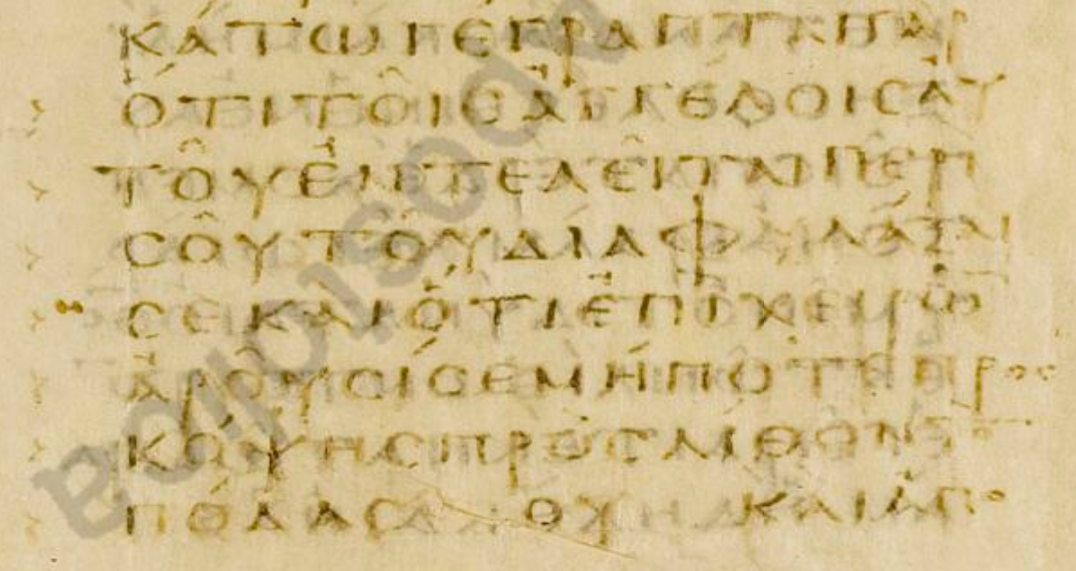
\includegraphics[width=0.8\textwidth]{../common/03_1310rb-Lk4:10-11}
\caption{A Lk 4:10-11 a Vatikáni kódexben}
\label{03-Lk4:10-11}
\end{center}
\end{figure}

Az írnok azonban felhívja figyelmünket arra, hogy idézetről van szó, és az akkori
szokásnak megfelelően a szöveg bal oldalán minden sorban egy $>$ jelet ír. (Ez a jelölés
gyakori a \textbf{01}-ben is, de ennél a szakasznál éppen hiányzik.)

A 91. zsoltárt ugyancsak megtaláljuk a \textbf{03}-ban (l. \ref{03-Ps90:11-12}. ábra),
itt is 90-es sorszámmal. Hasznunkra
lehet, hogy a zsoltárokat görög számokkal látták el, itt egy ún. \textit{koppa} szimbólum áll, ami
egy q-hoz hasonlít. Ez a része a kódexnek igen jól olvasható. Kiderül, hogy a \gr πασαις\hu\ (\textsc{minden}) szó
hiányzik a szövegből. Ezt a szót azonban a Lukács-szöveg sem tartalmazza a vizsgált
dokumentumok egyikében sem. Így ennek a szónak a hiánya az idézetek szempontjából irreleváns.

\begin{figure}
\begin{center}
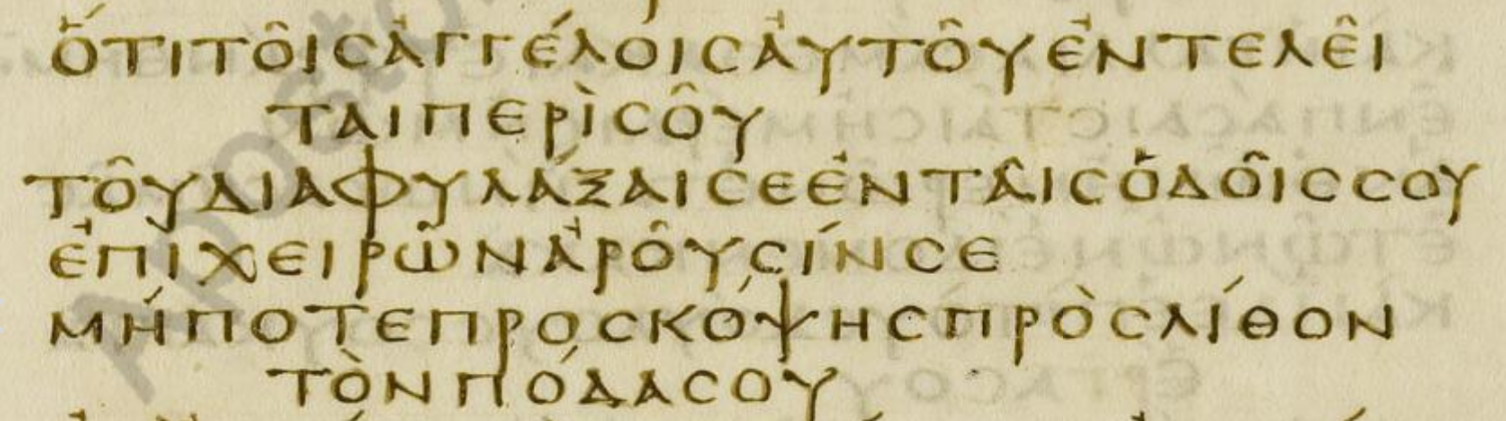
\includegraphics[width=0.8\textwidth]{../common/03_684lt-Ps90:11-12}
\caption{A 90/91. zsoltár 11-12. verse a Vatikáni kódexben, a 684. oldalon}
\label{03-Ps90:11-12}
\end{center}
\end{figure}

Végül az 5Móz 6:16-t keressük meg a lefényképezett kódexlapok között, melyet a 201. oldal
középső hasábjának közepén találunk (\ref{03-Deut6:16}. ábra). Arra lehetünk figyelmesek,
hogy a szöveg az ``Isten'' és ``Úr'' szavakat nem teljes alakjukban, csak első és utolsó
betűjükkel adja meg, fölöttük pedig egy vonallal köti össze őket. Ez is bevett szokás
a korabeli kéziratoknál. Egyéb különbség pedig nincsen az LXX szövegéhez képest.

\begin{figure}
\begin{center}
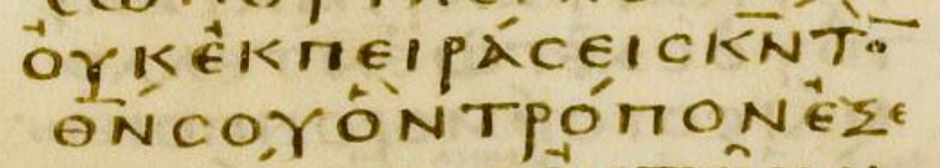
\includegraphics[width=0.8\textwidth]{../common/03_201mc-Deut6:16}
\caption{Az 5Móz 6:16 a Vatikáni kódexben}
\label{03-Deut6:16}
\end{center}
\end{figure}

\subsection{Az összehasonlítás haszna}

E bevezető fejezet végén kiemeljük, hogy a Septuaginta és a görög Újszövetség idézeteinek
objektív összehasonlítására tudományos és gyakorlati szempontból is igény van. Egy nemrégiben
készült doktori disszertáció \cite{SungKukKim} a Zsoltárok és a Jelenések közötti
kapcsolatokat gyűjti csokorba, felhívva a figyelmet arra, hogy a Jelenésekben nincs ugyan
\textit{formálisan idézett} zsoltár (2. o.), mégis számos gondolatra valamiféle
\textit{célzás} történik, melyeket a szerző \ref{celzas}. táblázat szerint osztályoz.
\begin{table}
\begin{tabular}{l | c | c}
& Szöveges egyezés & Kontextusbeli egyezés \\
\hline
Erős célzás & Nyilvánvaló & Nyilvánvaló\\
Valószínű célzás & Nem teljesen nyilvánvaló & Nyilvánvaló\\
Lehetséges célzás & Nem teljesen nyilvánvaló & Nem teljesen nyilvánvaló\\
Hatás & Megtalálható & Nem nyilvánvaló
\end{tabular}
\caption{Célzások kategorizálása S. K. Kim rendszerében}
\label{celzas}
\end{table}
A dolgozatban a szöveges egyezések mértékének meghatározására azonban nem találunk konkrét módszert.
Írásunk ebben az irányban próbál hiánypótló lenni, ill. az ehhez tartozó matematikai
és informatikai hátteret valamelyest megalapozni.

A Biblia megbízhatósága keresztény hitünk egyik alappilére. Tény, hogy Jézus és az ő követői is --
függetlenül attól, hogy korábban alapos teológiai képzésben részesültek (mint Pál) vagy nem
(mint a többi apostol) -- az Ószövetségre alapozták mondandójuk egy komoly részét.
A kereszténység hitelességének ezért az egyik próbája az, hogy írásos emlékeink összhangban
vannak-e egymással. Nem jelenti ez a kéziratok feltétlen betű szerinti egyezését, hiszen az isteni
tervnek része lehet az emberi tévesztés is, ami pl. másolási hibákat eredményezhet. De az is világos, hogy
a nyelv időbeli változása is hatással lehet az egyes kéziratok közötti eltérésekre. Az Írás
egyrészt tökéletességre int (Mt 5:48),
másrészt az emberi tökéletlenség nem akadálya annak, hogy Krisztus ereje megmutatkozzék
(2Kor 12:9). Harmadrészt Jézus kijelenti, hogy \textit{ég és föld elmúlnak, de az én igéim
nem múlnak el} (Lk 21:33), amint Ézsaiás is előre jelzi, hogy \textit{Istenünk beszéde
mindörökre megmarad} (Ézs 40:8).

Éppen ezért minden keresztény számára fontos, hogy a Biblia belső hivatkozásainak rendszeréről világos képünk legyen:
olyan, ami a tényeknek megfelel és tudományos szempontból is helytálló.

\section{Mi számít idézetnek?}

A Lk 4:9-12-ben megjelenő két ószövetségi utalás félreérthetetlenül idézetnek számít, mivel
mind a Sátán, mind Jézus konkrétan hangsúlyozza a forrást. Azonban nem minden idézetnek tűnő újszövetségi
szakasznál találunk ilyen konkrét referenciát, habár a szakasz idézet voltát
sok esetben egyértelműen jelzi az idézetet bevezető vagy magyarázó szöveg (itt: \textit{meg van írva} ill.
\textit{megmondatott}). Bizonyos esetekben a forrást is megnevezi a bevezető, esetleg a szerzőt
(vagy mindkettőt):
\begin{itemize}
\item Az ApCsel 13:33-ban olvassuk: \textit{Ahogyan meg van írva a második zsoltárban is$\ldots$}, a 13:34-ben
pedig a szerző pontosítása is megtörténik: \textit{Nektek váltom be a Dávidnak tett biztos, szent ígéreteket.}
\item A Róma 11:9 szerint: \textit{Dávid is ezt mondja$\ldots$}, habár itt nincs konkrét jelzés, hogy hol
található az eredeti szöveg. Ez egy gyakran előforduló idézési forma.
\item A János 13:18-ban olvassuk: \textit{$\ldots$ de be kell teljesednie az Írásnak}. Ez a fajta idézet
is gyakori.
\end{itemize}
Némely esetben nehéz eldönteni, hogy az Újszövetség csak \textit{utal} egy bizonyos ószövetségi szövegre,
vagy \textit{ténylegesen idézi} azt. Ha csak a Zsoltárok könyvére való utalásokat nézzük, akkor két olyan újszövetségi
igét is találunk, amelyek 50 betűnél is hosszabb egyezést mutatnak, de konkrét referencia nincs megadva:
\begin{itemize}
\item A Zsoltárok 2:9-re (\textit{Összetöröd őket vasvesszővel, szétzúzod, mint a cserépedényt!})
a Jelenések 2:27 utal: \textit{$\ldots$
hogy legeltesse őket vasvesszővel, törje őket össze, mint a cserépedényeket.}
\begin{center}
\begin{tabular}{p{5cm} p{5cm}}
LXX Zsolt 2:9 & SBLGNT Jel 2:27\\
\hline
& {\gr και}\\
{\gr \textcolor{red}{ποιμανει}ς } & 
{\gr \textcolor{red}{ποιμανει}}\\
{\gr \textcolor{blue}{αυτους εν ραβδω σιδηρα ως}}&
{\gr \textcolor{blue}{αυτους εν ραβδω σιδηρα ως} τα}\\
{\gr \textcolor{magenta}{σκευ}ος \textcolor{green}{κεραμ}εως \textcolor{orange}{συντρι}ψεις}
& {\gr \textcolor{magenta}{σκευ}η τα \textcolor{green}{κεραμ}ικα \textcolor{orange}{συντρι}βεται}\\
{\gr  αυτους}&
\end{tabular}
\end{center}
\hu
Szigorú értelemben a két szakasz csak 21 karakter hosszan egyezik meg teljesen, betű szerint,
de az apró eltéréseket nem számítva jóval hosszabb az egyezés.
\item A Zsolt 146:6 első szavaira (\textit{aki az eget és a földet alkotta, meg a tengert, és ami csak bennük van})
az ApCsel 4:24 (\textit{teremtetted az eget és a földet, a tengert és mindent, ami bennük van}) és 14:15 
(\textit{teremtette az eget és a földet, a tengert és mindent, ami bennük van}) is utal, ahogyan ezt
a görög szövegek is sugallják:
\begin{center}
\begin{tabular}{p{3.3cm} p{3.3cm} p{3.3cm}}
LXX & SBLGNT & SBLGNT\\
Zsolt 146:6 & ApCsel 4:24 & ApCsel 14:15\\
\hline
{\gr 
 \textcolor{red}{ποιησ}αντα} &
{\gr 
 \textcolor{red}{ποιησ}ας} &
{\gr 
 ε\textcolor{red}{ποιησ}εν}\\
{\gr \textcolor{blue}{τον ουρανον}}&
{\gr \textcolor{blue}{τον ουρανον}}&
{\gr \textcolor{blue}{τον ουρανον}}\\
{\gr \textcolor{blue}{και την γην} \textcolor{magenta}{την}} &
{\gr \textcolor{blue}{και την γην} και \textcolor{magenta}{την}} &
{\gr \textcolor{blue}{και την γην} και \textcolor{magenta}{την}}\\
{\gr \textcolor{magenta}{θαλασσαν και παντα τα εν αυτοις}}&
{\gr \textcolor{magenta}{θαλασσαν και παντα τα εν αυτοις}}&
{\gr \textcolor{magenta}{θαλασσαν και παντα τα εν αυτοις}}
\end{tabular}
\end{center}
\hu
A két újszövetségi szakasz környékén azonban nem találjuk annak említését, hogy az Ószövetségből
lenne a kérdéses szöveg átvéve. Így szigorú értelemben ezek az egyezések nem tekinthetők
idézetnek, hiába a hosszú, szinte betű szerinti egyezés.
\end{itemize}
Van néhány további zsoltárszakasz, amelyről itt említést kell tennünk. Ilyen pl. a Zsolt 31:5
(a maszoréta szövegben ez a Zsolt 31:6:
\textit{Kezedre bízom lelkemet$\ldots$}), amire Jézus a kereszten
utal a Lk 23:46-ban (\textit{$\ldots$a te kezedbe teszem le az én lelkemet}), de nincs feltüntetve,
hogy Jézus itt valóban az ószövetségi Írásra gondol -- ez a szakasz 34 karakternyi egyezést jelent.
További példa a Zsolt 118:26 (\textit{Áldott, aki az ÚR nevében jön!}), amely 36 karakter hosszú,
és betű szerint ugyanígy található meg a Mt 21:9-ben, a Mt 23:39-ben, a Mk 11:9-ben,
a Lk 13:35-ben, a Lk 19:38-ban, illetve a Jn 12:13-ban. A szövegkörnyezetek alapján előfordulhat,
hogy az ezt kiáltó sokaság valóban a 118. zsoltárt tudatosan szavalta, de ezt nem támasztja alá a kontextus.

Ezen kívül számos, a fenti szövegeknél rövidebb, betű szerinti egyezés található, amelyeket
a kontextus alapján nem azonosíthatunk idézetként, de előfordulhat, hogy az újszövetségi szerző
-- akár tudatosan, akár nem -- utalni akart az Ószövetség valamely szakaszára. Olyan is előfordul,
hogy egy ószövetségi kifejezést az újszövetségi szerző egyszerűen csak felhasznál, azért, hogy
mondanivalóját kifejezhesse.

Ebben a tanulmányban a továbbiakban \textit{idézeten} csak olyan ó- és újszövetségi szakaszpárokat értünk,
ahol az újszövetségi szakasz környékén konkrét említés történik arról,
hogy idézetről van szó. Azoknál a szakaszpároknál,
ahol ilyen említés nincs, de a kontextus valamelyest támogatja a kapcsolatot, \textit{utalás}ról beszélünk.
A többi esetben \textit{véletlen egyezés}ről fogunk beszélni.

Az idézeteket többé-kevésbé objektív módon meg lehet határozni, míg az utalásoknál valamennyire szürke
zónában vagyunk, és némely teológus bizonyos szövegpároknál esetleg nem látja
a kapcsolatot bizonyítottnak. Tanulmányunkban az idézetek gépi módon történő beazonosítására törekszünk.
Nyilvánvaló, hogy ehhez a kontextus valamiféle értelmezése is szükséges, így egy egyszerű,
a görög nyelvet értelmezni nem tudó gépi algoritmus nem adhat teljes értékű kimenetet.

Arra azonban van mód, hogy egy gépi algoritmus idézeteket, utalásokat és véletlen egyezéseket \textit{egyszerre}
tárjon fel anélkül, hogy a pontos kategóriát meghatározná. Látni fogjuk, hogy még a kontextus
megértése nélkül is adhatók algoritmusok, amelyek még a pontos kategóriára is jó tippet adhatnak,
ha nem is adhatnak teljes értékű kimenetet.


\section{Szövegek gépi összehasonlítása}

Hasznos lesz, ha a \gr σ  \hu\ és \gr ς\hu\ betűket nem különböztetjük meg. Így csak 24 betűvel kell dolgoznunk.
Ezt megtehetjük, mivel a korai kéziratokban nincs különbség eközött a két betű között.

Bibliai \textit{könyv}ön a továbbiakban egy olyan karaktersorozatot értünk, amely a görög ábécé 24
betűjéből áll. Egy könyvnek tekintjük a szokásosan könyvként ismert bibliai szövegeket,
így az 1Móz-t, 2Móz-t és így tovább. A Zsoltárok könyvét 150 külön könyvként fogjuk tekinteni,
mivel ezekre az Újszövetség is külön egységenként tekint (l. ApCsel 13:33).
Erre az alapvetésre azért van szükség, mert feltételezzük, hogy egy idézet csupán egy és nem több
könyvből származik -- ugyanez nem feltétlenül lenne elmondható akkor, ha fejezetekre osztva
vizsgálnánk a szövegeket: ez önkényes döntés lenne, és az idézetek akár fejezethatárokon is átívelhetnének.
(Valójában a fejezethatárok nem is feltétlenül egységesek a különböző bibliafordításokban.)

Egy pillanatra eszünkbe juthat, hogy a Biblia esetében bizonyos héber nyelvű könyvekben van értelme vershatárokról is
beszélni, hiszen vagy azonos, vagy egymást követő betűkkel kezdődnek bizonyos versek vagy rész-versek a héber
eredetiben. Ahogyan a korábbiakban már utaltunk rá: a zsoltárok közül többek között a 119. és a 145.,
továbbá a Jeremiás siralmai egy része, valamint a Példabeszédek könyvének utolsó versei is ilyenek jellegzetességet
hordoznak.
A görög nyelvű szövegben azonban ezek a szabályosságok hiányoznak, így a vershatároknak
a jelentősége kevésbé tűnik fontosnak. Másrészt az idézetek gyakran átívelnek a vershatárokon.
Így pl. a 69. zsoltár 10. versénél az első felet (\textit{Mert a házad
iránti féltő szeretet emészt}) a Jn 2:17 idézi, míg a 2. felet (\textit{rám hull a gyalázat, ha téged gyaláznak})
a Róm 15:3, világos tehát, hogy verseken belüli részekre is mutathatnak idézetek. Továbbá, pl. a 16. zsoltár
8-11. versét az ApCsel 2,25-28 idézi, de a 11. vers utolsó szavait nem. Célszerűbbnek látszik tehát
a vershatároktól teljesen elvonatkoztatni, és inkább adott betűtől adott betűig terjedő szakaszokat vizsgálni.
Ezért tehát a szokásos versbeosztást a további algoritmusokban teljesen figyelmen kívül hagyjuk.

Legyen tehát adott egy $A$ ábécé: $A=\{\alpha,\beta,\ldots,\omega\}$. Tekintsünk egy adott bibliát
vagy bibliafordítást, és vegyük annak egy könyvét a fent leírt módon. Amennyiben korrektor módosította
a szöveget egy vagy több helyen, minden esetben döntsük el, hogy melyik szövegvariánst használjuk.
(Egy vizsgálat során tehát mindig egyetlen szövegvariánssal dolgozunk. A plauzibilis bibliák esetében
mindig egyetlen szövegvariáns van, ilyen biblia lesz az általunk használt LXX és SBLGNT is.)
A kiválasztott könyvet $B$-vel fogjuk jelölni,
ahol $B\in A^n$, ahol $A^n$ egy $n$ szorzatból álló Descartes-hatvány. Feltesszük tehát, hogy a könyv
$n$ karakterből áll. Vagyis $B=(b_1,b_2,\ldots,b_n)$, ahol minden $b_i$ elem $A$-beli:
$b_i\in A$, $i=1,2,\ldots,n$.

Legyen adott továbbá a $B$ könyvnek egy bizonyos $m$ hosszú $T$ szövege ($m\in\mathbb{N}$), valamely $T\in A^m$, ahol
$T=(t_1,t_2,\ldots,t_m)$, melyre $t_1=b_k,t_2=b_{k+1},\ldots,t_m=b_{k+m-1}$ valamely $k\in\mathbb{N}$-re. A
$T$ szövegre jellemző $k$ számot $T$-nek $B$-beli pozíciójának nevezzük és $p(T,B)$-vel jelöljük.
Az $m$ hosszot $|T|$-vel jelöljük.

\subsection{Pontos egyezés}

\subsubsection{Alapfogalmak}

Először a pontos egyezés matematikai hátterét írjuk le.

Azt mondjuk, hogy egy $T_1=(u_1,u_2,\ldots,u_m)\in A^{m}$ szöveg \textit{megegyezik} egy
egy $T_2=(v_1,v_2,\ldots,v_m)\in A^{m}$ szöveggel, ha $u_1=v_1, u_2=v_2, \ldots u_m=v_m$.
Ezt úgy jelöljük, hogy $T_1=T_2$.

Azt mondjuk, hogy egy $T_1=(u_1,u_2,\ldots,u_{m_1})\in A^{m_1}$ szöveg \textit{része}
egy $T_2=(v_1,v_2,\ldots,v_{m_1})\in A^{m_2}$ szövegnek ($m_1,m_2\in\mathbb{N}$),
ha $m_1\leq m_2$, valamint $u_1=v_{k},u_2=v_{k+1},\ldots,u_{m_1}=v_{k+m_1-1}$ valamely $k\in\mathbb{N}$-re.
A ``része lenni'' relációt $T_1\subseteq T_2$-vel jelöljük. Triviálisan fennáll minden
$T$ szövegre, hogy $T\subseteq B$, amennyiben a $B$ könyvnek egy szövege $T$.
Amennyiben $m_1<m_2$, úgy a $T\subset B$ jelölést is használjuk.
A $T_1\equiv T_2$ jelölést alkalmazzuk továbbá, ha $m_1=m_2$.

Tekintsünk egy ószövetségi $B$ könyvet és abban egy $T$ szöveget. Azt mondjuk, hogy egy $T\subset B$ szöveg
\textit{egyedi} a $B$ könyvben, ha valamely $T'\subset B$-ből $p(T',B)=p(T,B)$ következik.

Legyen $T_1,T_2\in B$, ahol $B$ egy adott ószövetségi könyv. Azt mondjuk, hogy $T_1$ a $T_2$
\textit{igehelyen belül van}, ha $T_1\subset T_2$, $p(T_1,B)\geq p(T_2,B)$ és $p(T_1,B)+|T_1|\leq p(T_2,B)+|T_2|$.
Az ``igehelyen belül lenni'' relációt $T_1\leq T_2$-vel jelöljük. Triviálisan fennáll minden
$T$ szövegre, hogy $T\leq B$, amennyiben $T\subseteq B$. Amennyiben $T_1\not\equiv T_2$, úgy
a $T_1<T_2$ jelölést is alkalmazzuk. Világos, hogy $T\subset B$-ből $T<B$ is következik.

Tekintsük most az ószövetségi könyvek $O=\{B_1,B_2,\ldots,B_l\}$ halmazát ($l\in\mathbb{N}$) egy adott kéziraton
vagy bibliafordításon belül.
Tekintsünk ezen kívül egy ószövetségi $B$ könyvet ($B\in O$) és abban egy $T$ szöveget ($T\in B$). Azt mondjuk, hogy
$T$ \textit{egyedi} az $O$ ószövetségi könyvekben, ha egyedi a $B$ könyvben, valamint egyetlen más $B'$ könyvben
sem áll fenn $T\subseteq B'$.

Legyen adott ószövetségi könyvek $O=\{B_1,B_2,\ldots,B_l\}$ halmaza ($l\in\mathbb{N}$) egy adott kéziraton 
vagy bibliafordításon belül.
Legyen $T$ a $B\in O$ könyv valamely szövege, valamint tegyük fel, hogy $T$ egyedi az $O$ ószövetségi könyvekben.
Legyen továbbá adott egy $N$ újszövetségi könyv és annak egy $U\subseteq N$ szövege.
Azt mondjuk, hogy $U$ \textit{lehetséges idézet}, továbbá $U$ \textit{idézheti} a $T$ idézett szöveget,
ha $T=U$. Azt mondjuk továbbá, hogy $U$ maximális lehetséges idézet,
ha minden olyan $U'$-re, amelyre $U<U'$, $U'$ nem lehetséges idézet.

\paragraph{Példák}

\begin{enumerate}
\item Tekintsük az LXX-et. Ebben legyen $B$ az 5Móz-hez tartozó matematikai objektum. $|B|=108557$, vagyis ennyi
karakterből áll a kérdéses könyv. A $T=\textrm{\gr ουκεκπειρασειςκυριοντονθεονσου\hu}$ szöveg a 23212.
pozíción kezdődik $B$-ben, vagyis $p(T,B)=23212$, hossza 30 karakter, tehát $|T|=30$. $T$ egyedi $B$-ben,
de az egész LXX-ben is.

Legyen ezen kívül $N$ a Lk-hoz tartozó matematikai objektum az SBLGNT-ből. $|N|=94627$. $p(T,N)=13792$.
$T$ tehát lehetséges idézet,
valamint maximális lehetséges idézet, mert a Lk 4:12-nek ezt a néhány szavát tartalmazó, az igehelyet magát
is befoglaló szakasz nincs a Lukácsban, ami az Ószövetségben is jelen lenne.

A fentieket a \texttt{bibref} szoftverben az olvasó is ellenőrizheti:
\begin{lstlisting}
>> addbooks
>> lookup1 LXX Deuteronomy 6:16 6:16-33
Stored internally as oykekpeiraseiskyriontonueonsoy.
>> length1
Length of text 1 is 30.
>> find1 LXX
Found in Deuteronomy 6:16 6:16 (book position 23212)
1 occurrences.
>> find1 SBLGNT 
Found in Matthew 4:7+28 4:7 (book position 6621)
Found in Luke 4:12+39 4:12 (book position 13792)
2 occurrences.
\end{lstlisting}
(A fent használt jelölésekkel egy bibliaversen belüli betű szerinti pontosításokat adhatunk meg.
Így pl. az \texttt{LXX Deuteronomy 6:16 6:16-33} kód jelentése: az LXX bibliakiadásban az 5Móz 6:16 verse,
amelynek végéről 33 betűt elhagyunk. Másrészt a \texttt{Luke 4:12+39 4:12} jelentése: A Lk 4:12 verse
az első 39 betű elhagyásával.)

\item Tekintsük az LXX-et. Ebben legyen $B$ a 91. zsoltár, valamint
$$T=\textrm{\gr τοιςαγγελοιςαυτουεντελειταιπερισουτουδιαφυλαξαισε\hu}.$$ $|T|=49$. $T$ egyedi az egész LXX-ben.

Legyen továbbá $N$ ismét a Lk-hoz tartozó objektum az SBLGNT-ből. $p(T,N)=13646$. $T$ tehát lehetséges idézet,
de nem maximális, ugyanis a Lk 4:10-nek ezt a szakaszát tartalmazó
$$T'=\textrm{\gr οτιτοιςαγγελοιςαυτουεντελειταιπερισουτουδιαφυλαξαισε\hu}$$
szövegre $T<T'$ teljesül, továbbá $T'$ lehetséges idézet $B$-ben. $T'$ azonban már maximális.

Ez a példa a \texttt{bibref} programmal így ellenőrizhető:

\begin{lstlisting}
>> lookup1 LXX Psalms 91:11+3 91:11-20
Stored internally as toisaggeloisaytoyenteleitaiperisoytoydiafylajaise.
>> find1 LXX
Found in Psalms 91:11+3 91:11 (book position 107359)
1 occurrences.
>> find1 SBLGNT
Found in Luke 4:10+15 4:10 (book position 13646)
1 occurrences.
>> extend LXX SBLGNT Luke 4:10+15 4:10
Extended match is LXX Psalms 91:11 91:11-20 = SBLGNT Luke 4:10+12 4:10 (otitoisaggeloisaytoyenteleitaiperisoytoydiafylajaise, length 52).
\end{lstlisting}

\end{enumerate}

\subsubsection{Pontos lehetséges idézetek}

Legyen adott ószövetségi könyvek $O=\{B_1,B_2,\ldots,B_l\}$ halmaza ($l\in\mathbb{N}$) egy adott kéziraton 
vagy bibliafordításon belül.
Legyen $T$ a $B\in O$ könyv valamely szövege, valamint tegyük fel, hogy $T$ egyedi az $O$ ószövetségi könyvekben.
Ekkor világos, hogy létezik egy olyan $T'<T$ szöveg, mely már nem egyedi: szélsőséges esetben $T'$ egyetlen
betűből áll, és mivel feltételezhetően minden betű szerepel minden bibliában, ilyen $T'$ megadható.
Mindebből az is következik, hogy lesz olyan $T''<T$, amely minimálisan egyedi, vagyis bármely
$T'''<T''$ esetén $T'''$ nem egyedi, de $T''$ igen.

\paragraph{Példa}

Tekintsük az LXX-ben lévő 82. zsoltár 6. versét. Ismert, hogy ennek elejét a Jn 10:34 vége idézi:
\gr εγω ειπα θεοι εστε\hu. Ez a szöveg egyedi az LXX-ben, de csak önmagában a második két szó még nem az,
mert az Ézs 41:23 végén is jelen van:
\begin{lstlisting}
>> lookup1 LXX Psalms 82:6+7 82:6-20
Stored internally as ueoieste.
>> find1 LXX
Found in Psalms 82:6+7 82:6 (book position 96144)
Found in Isaiah 41:23+51 41:23 (book position 82752)
2 occurrences.
\end{lstlisting}
Azonban még egy betűt hozzávéve ehhez a két szóhoz már egyedi szöveget kapunk:
\begin{lstlisting}
>> lookup1 LXX Psalms 82:6+6 82:6-20
Stored internally as aueoieste.
>> find1 LXX
Found in Psalms 82:6+6 82:6 (book position 96143)
1 occurrences.
\end{lstlisting}
A fenti jelölésekhez igazodva itt $T=\textrm{\gr εγωειπαθεοιεστε\hu}$,
$T'=\textrm{\gr θεοιεστε\hu}$, $T''=\textrm{\gr αθεοιεστε\hu}$.

A minimálisan egyedi szövegek megtalálása nagy segítséget fog nyújtani az idézetek beazonosításában.
Tekintsünk ugyanis egy $T\subseteq B\in O$ szöveget. Az ebben lévő minimálisan egyedi szövegeket
az \ref{algo-min-egyedi}. algoritmussal találhatjuk meg.

\begin{algorithm}
\caption{Algoritmus egy $T=(t_1,t_2,\ldots,t_\ell)$ szöveg összes minimálisan egyedi szövegének megtalálásához}
\label{algo-min-egyedi}
\begin{algorithmic}[1]
\Procedure{minunique}{$T$}
 \State $\ell \gets |T|$
 \For {$i \gets 1$-től $\ell$-ig}
  \For {$j \gets 1$-től $\ell-i$-ig}
   \State {$U_{i,j}=-1$}
  \EndFor
 \EndFor

 \For {$i \gets 1$-től $\ell$-ig}
  \For {$j \gets 1$-től $\ell-i$-ig}
   \If {$i>1 \wedge (U_{i-1,j}>0 \vee U_{i-1,j+1}>0$)}
    \State {$U_{i,j} \gets \textcolor{blue}{2}$}
   \Else
    \State {$T' \gets (t_j,t_{j+1},\ldots,t_{j+i-1})$}
    \If {$T'$ egyedi}
      \State {$U_{i,j} \gets \textcolor{red}{1}$}
      \State \textbf{írd ki} {$T'$}-t
    \Else
     \State {$U_{i,j} \gets 0$}
    \EndIf
   \EndIf
  \EndFor
 \EndFor
\EndProcedure
\end{algorithmic}
\end{algorithm}

Az algoritmus áttekintéséhez tekintsük az \textit{abcdef} szöveget, melyről tudjuk, hogy \textit{ab}
ill. \textit{cde} minimálisan egyediek. Készítsük el az alábbi táblázatot:
\begin{center}
\begin{tabular}{r|lc|clc|clc|l|l|l|}
  & 1 & & & 2&  & & 3 & & 4 & 5 & 6\\
\hline
1 & a & & & b & & & c & & d & e & f\\
\hline
2 & \textcolor{red}{ab} & \textcolor{red}{$\downarrow$} & & bc & & & cd & & de & ef & \\
\hline
3 & \textcolor{blue}{abc} & \textcolor{blue}{$\downarrow$} & & bcd & & \textcolor{red}{$\swarrow$} & \textcolor{red}{cde} &  \textcolor{red}{$\downarrow$} & def & & \\
\hline
4 & \textcolor{blue}{abcd} & \textcolor{blue}{$\downarrow$} & \textcolor{blue}{$\swarrow$} & \textcolor{blue}{bcde} & \textcolor{blue}{$\downarrow$} & \textcolor{blue}{$\swarrow$} & \textcolor{blue}{cdef} & & & & \\
\hline
5 & \textcolor{blue}{abcde} & \textcolor{blue}{$\downarrow$} & \textcolor{blue}{$\swarrow$} & \textcolor{blue}{bcdef} & & & & & & & \\
\hline
6 & \textcolor{blue}{abcdef} & & & & & & & & & & \\
\hline
\end{tabular}
\end{center}
%\label{abcde}
Általánosan igaz, hogy minden egyedi szöveg alatt és a tőle balra-le álló cella szintén egyedi szöveget takar. Így a táblázatot
fentről-lefelé, ezen belül balról-jobbra kitöltve csak a minimálisan egyedi szövegek ismeretében gyorsan megadható, hogy
mely szövegek egyediek: a pirosak (melyek minimálisak) és a kékek (melyek nem-minimálisak).
A fenti táblázat egy alternatív, ``kisebb helyen elférő'' változata a következő:
\begin{center}
\begin{tabular}{c c c c c c}
\textcolor{green}{a} & b & \textcolor{green}{c} & d & e & f \\
\textcolor{red}{b} & c & \textcolor{green}{d} & e & f & \\
\textcolor{blue}c & d & \textcolor{red}{e} & f & & \\
\textcolor{blue}d & \textcolor{blue}e & \textcolor{blue}f& & &\\
\textcolor{blue}e & \textcolor{blue}f & & & &\\
\textcolor{blue}f & & & & &
\end{tabular}
\end{center}
Itt függőlegesen kell kiolvasnunk az egyes szövegeket, fentről lefele, a piros betűvel bezárólag.
A fenti módszernek megfelelően elkészítjük
a Zsolt 82:5-6 versének közbülső, \gr γης
εγω ειπα θεοι εστε και\hu\ szavaihoz tartozó táblázatot (a könnyebb olvashatóság
kedvéért latin betűkkel):

\begin{center}
\scalebox{0.8}{
\begin{tabular}{c c c c c c c c c c c c c c c c c c c c c}
g&\textcolor{green}h&\textcolor{green}s&e&g&v&\textcolor{green}e&\textcolor{green}i&\textcolor{green}p&\textcolor{green}a&u&\textcolor{green}e&o&i&e&s&t&e&k&a&i \\
h&\textcolor{green}s&\textcolor{green}e&g&v&e&\textcolor{green}i&\textcolor{green}p&\textcolor{green}a&\textcolor{green}u&e&\textcolor{green}o&i&e&s&t&e&k&a&i& \\
s&\textcolor{green}e&\textcolor{green}g&v&e&i&\textcolor{green}p&\textcolor{green}a&\textcolor{green}u&\textcolor{green}e&o&\textcolor{green}i&e&s&t&e&k&a&i&& \\
e&\textcolor{green}g&\textcolor{green}v&e&i&p&\textcolor{green}a&\textcolor{green}u&\textcolor{green}e&\textcolor{green}o&i&\textcolor{green}e&s&t&e&k&a&i&&& \\
g&\textcolor{green}v&\textcolor{green}e&i&p&a&\textcolor{red}u&\textcolor{red}e&\textcolor{red}o&\textcolor{green}i&e&\textcolor{green}s&t&e&k&a&i&&&& \\
v&\textcolor{green}e&\textcolor{green}i&p&a&\textcolor{blue}u&\textcolor{blue}e&\textcolor{blue}o&\textcolor{blue}i&\textcolor{red}e&s&\textcolor{green}t&e&k&a&i&&&&& \\
e&\textcolor{green}i&\textcolor{green}p&a&\textcolor{blue}u&\textcolor{blue}e&\textcolor{blue}o&\textcolor{blue}i&\textcolor{blue}e&\textcolor{blue}s&t&\textcolor{green}e&k&a&i&&&&&& \\
i&\textcolor{red}p&\textcolor{red}a&\textcolor{blue}u&\textcolor{blue}e&\textcolor{blue}o&\textcolor{blue}i&\textcolor{blue}e&\textcolor{blue}s&\textcolor{blue}t&e&\textcolor{red}k&a&i&&&&&&& \\
\textcolor{blue}p&\textcolor{blue}a&\textcolor{blue}u&\textcolor{blue}e&\textcolor{blue}o&\textcolor{blue}i&\textcolor{blue}e&\textcolor{blue}s&\textcolor{blue}t&\textcolor{blue}e&\textcolor{blue}k&\textcolor{blue}a&i&&&&&&&& \\
\textcolor{blue}a&\textcolor{blue}u&\textcolor{blue}e&\textcolor{blue}o&\textcolor{blue}i&\textcolor{blue}e&\textcolor{blue}s&\textcolor{blue}t&\textcolor{blue}e&\textcolor{blue}k&\textcolor{blue}a&\textcolor{blue}i&&&&&&&&& \\
\textcolor{blue}u&\textcolor{blue}e&\textcolor{blue}o&\textcolor{blue}i&\textcolor{blue}e&\textcolor{blue}s&\textcolor{blue}t&\textcolor{blue}e&\textcolor{blue}k&\textcolor{blue}a&\textcolor{blue}i&&&&&&&&&& \\
\textcolor{blue}e&\textcolor{blue}o&\textcolor{blue}i&\textcolor{blue}e&\textcolor{blue}s&\textcolor{blue}t&\textcolor{blue}e&\textcolor{blue}k&\textcolor{blue}a&\textcolor{blue}i&&&&&&&&&&& \\
\textcolor{blue}o&\textcolor{blue}i&\textcolor{blue}e&\textcolor{blue}s&\textcolor{blue}t&\textcolor{blue}e&\textcolor{blue}k&\textcolor{blue}a&\textcolor{blue}i&&&&&&&&&&&& \\
\textcolor{blue}i&\textcolor{blue}e&\textcolor{blue}s&\textcolor{blue}t&\textcolor{blue}e&\textcolor{blue}k&\textcolor{blue}a&\textcolor{blue}i&&&&&&&&&&&&& \\
\textcolor{blue}e&\textcolor{blue}s&\textcolor{blue}t&\textcolor{blue}e&\textcolor{blue}k&\textcolor{blue}a&\textcolor{blue}i&&&&&&&&&&&&&& \\
\textcolor{blue}s&\textcolor{blue}t&\textcolor{blue}e&\textcolor{blue}k&\textcolor{blue}a&\textcolor{blue}i&&&&&&&&&&&&&&& \\
\textcolor{blue}t&\textcolor{blue}e&\textcolor{blue}k&\textcolor{blue}a&\textcolor{blue}i&&&&&&&&&&&&&&&& \\
\textcolor{blue}e&\textcolor{blue}k&\textcolor{blue}a&\textcolor{blue}i&&&&&&&&&&&&&&&&& \\
\textcolor{blue}k&\textcolor{blue}a&\textcolor{blue}i&&&&&&&&&&&&&&&&&& \\
\textcolor{blue}a&\textcolor{blue}i&&&&&&&&&&&&&&&&&&& \\
\textcolor{blue}i&&&&&&&&&&&&&&&&&&&& \\
\end{tabular}
}
\end{center}

Ezt az eredményt a \texttt{bibref} programmal is ellenőrizhetjük:

\begin{lstlisting}
>> lookup1 LXX Psalms 82:5+72 82:6-17
Stored internally as ghsegveipaueoiestekai.
>> minunique1 LXX
Text eipau is minimal unique.
Text ipaue is minimal unique.
Text paueo is minimal unique.
Text aueoie is minimal unique.
Text hsegveip is minimal unique.
Text segveipa is minimal unique.
Text eoiestek is minimal unique.
\end{lstlisting}

Ebben a fázisban már megkereshetőek azok a potenciális újszövetségi igehelyek,
amelyek a kapott minimálisan egyedi szövegeket idézik. A \texttt{bibref} program
ebben is segítséget ad, pl. a latin írással megadott ``eipau'' szöveg az
Újszövetségben 4 helyen is előfordul.

\begin{lstlisting}
>> latintext2 eipau
Stored.
>> find2 SBLGNT 
Found in Luke 24:26+11 24:26 (book position 92671)
Found in John 10:34+58 10:34 (book position 35754)
Found in Acts 17:3+40 17:3 (book position 55405)
Found in Acts 26:23 26:23 (book position 86624)
4 occurrences.
\end{lstlisting}

Ezek közül a János 10:34 találatra számítottunk is. A másik 3 viszont véletlen egybeesés,
és csak erre az 5 betűre vonatkozik.
A későbbiekben látni fogjuk, hogy a tényleges idézetek 5 betűnél általában jóval hosszabbak,
így ezek a téves találatok többnyire gépi úton is kiszűrhetőek.

E szakasz végén röviden igazoljuk az algoritmus helyességét:
\begin{theorem}
Az \ref{algo-min-egyedi}. algoritmus pontosan azonosítja a $T$ szöveg összes egyedi rész-szövegét,
mind az egyedieket és azon belül a minimálisakat.
\end{theorem}
\begin{proof}
Megmutatjuk, hogy az algoritmus végén $U_{i,j}$ a helyes értéket
tartalmazza minden $1\leq i\leq |T|$, $1\leq j\leq |T|$, $i+j\leq |T|+1$ esetén,
vagyis 0-t tartalmaz, ha a $(t_j,t_{j+1},\ldots,t_{j+i-1})$ szöveg nem egyedi,
\textcolor{red}{1}-et, ha minimálisan egyedi, és \textcolor{blue}{2}-t, ha egyedi (de nem minimálisan).

$i$ szerinti teljes indukciót alkalmazunk. Legyen $i=1$, ekkor $U_{1,j}$ az algoritmus
13. ill. 16. sora szerint \textcolor{red}{1}-et vagy 0-t vesz fel a $t_j$ betű egyediségének
megfelelően. Legyen most $1<i\leq |T|$ tetszőleges. Az $U_{i,j}$ által leírt
$(t_j,t_{j+1},\ldots,t_{j+i-1})$ szöveg akkor és csak akkor
egyedi, ha az $U_{i-1,j}$ vagy $U_{i-1,j+1}$ által leírt
$(t_j,t_{j+1},\ldots,t_{j+i-2})$ vagy $(t_{j+1},t_{j+2},\ldots,t_{j+i-1})$
szövegek
\begin{itemize}
\item valamelyike egyedi, ebben az esetben az algoritmus 9. sora szerint
$(t_j,t_{j+1},\ldots,t_{j+i-1})$ egyedi, de nem minimálisan, így
az $U_{i,j}=\textcolor{blue}{2}$ érték helyes,
\item egyike sem egyedi, de a $(t_j,t_{j+1},\ldots,t_{j+i-1})$ szöveg már egyedi,
így ezen szöveg minimálisan is egyedi, tehát az $U_{i,j}=\textcolor{red}{1}$
érték helyes (13. sor).
\end{itemize}
A maradék esetben a 16. sor szerint $U_{i,j}$-be 0 kell kerüljön, mert a
hozzá tartozó szöveg nem egyedi.
\end{proof}

Az \ref{algo-min-egyedi}. algoritmus jelentősége abban áll, hogy a nem minimálisan egyedi
szövegeknél nem kell az általában nagy számítási igénnyel járó egyediség-ellenőrzést
végigfuttatni. A 82. zsoltárban fent ellenőrzött 21 betűs szakasz esetében a 231 egyediség-ellenőrzésből
csak 124-re kellett végigszámolni. A további számításokat pedig a 114 egyedi szöveg helyett
csak a 7 minimálisan egyedi szövegre kell elvégezni.

A fentiek segítségével egy további algoritmus adható, hogy egy ószövetségi szövegben megkeressük
az összes olyan szövegrészt, amelyeket az Újszövetség idéz. A találatok között lehetnek
ugyan véletlen egybeesések, azonban a módszer teljes abban az értelemben, hogy egyetlen
lehetséges idézet sem marad ki. A módszert a \ref{algo-osz-uszi-ref}. algoritmus részletezi, melyben a már korábban
említett \textsc{extend} eljárással egy lehetséges idézetet maximálizálunk.

\begin{algorithm}
\caption{Algoritmus egy $T$ ószövetségi ($O$) szöveg összes
újszövetségi ($N$) lehetséges idézetének megtalálásához}
\label{algo-osz-uszi-ref}
\begin{algorithmic}[1]
\Procedure{getrefs}{$T$}
 \For {$m \gets \textsc{minunique}(T)$}
  \For {$B_2\in N$}
   \For {$T'\subseteq B_2$}
    \If {$T'=T$}
     \State {$T'' \gets \textsc{extend}(T')$}
      \For {$B_1\in O$}
       \For {$T'''\subseteq B_1$}
        \If {$T'''=T''$}
         \State \textbf{írd ki} {$T''$}-t
        \EndIf
       \EndFor
      \EndFor
    \EndIf
   \EndFor
  \EndFor
 \EndFor
\EndProcedure
\end{algorithmic}
\end{algorithm}

Az algoritmust (ill. annak rendezett eredményét) az alábbi \texttt{bibref}-kimenet mutatja:

\begin{lstlisting}
>> getrefs SBLGNT LXX Psalms 91:11
LXX Psalms 91:11+24 91:11-41 = SBLGNT Revelation_of_John 11:8+54 11:8-55 (length=7, pos1=107379)
LXX Psalms 91:11+24 91:11-40 = SBLGNT Acts 10:32+45 10:32-51 (length=8, pos1=107379)
LXX Psalms 91:11+24 91:11-40 = SBLGNT Acts 10:5+57 10:5-4 (length=8, pos1=107379)
LXX Psalms 91:11 91:11-63 = SBLGNT Romans 8:28+9 8:28-62 (length=9, pos1=107355)
LXX Psalms 91:11+25 91:11-38 = SBLGNT Luke 17:2+32 17:2-73 (length=9, pos1=107380)
LXX Psalms 91:11+2 91:11-51 = SBLGNT Matthew 25:41+95 25:42-56 (length=19, pos1=107357)
LXX Psalms 91:11 91:11-35 = SBLGNT Matthew 4:6+54 4:6-55 (length=37, pos1=107355)
LXX Psalms 91:11 91:11-20 = SBLGNT Luke 4:10+12 4:10 (length=52, pos1=107355)
\end{lstlisting}

Örvendetes, hogy a Lk 4:10 mint maximális lehetséges idézet jelent meg, azonban vannak további találatok is,
amelyek rövidebbek, és kétségkívük csak véletlen egyezések. A 37 hosszú Mt 4:6-beli egyezés viszont
helyes, mivel Máté szövege ugyancsak idézi a 91. zsoltárt. A Mt 25:41-ben található 19
betűnyi egyezés azonban tartalmilag csak annyiban egyezik, hogy az ``Ő angyalai''-ról szól.

Nehéz dolog annak meghatározása, hogy hány betűnél húzzuk meg a határt, ami fölött már biztos
egyezésről van szó. A Zsolt 82:6-ra való hivatkozásra keresés a 15 betűs Jn 10:34 igehelyet
jól beazonosítja, ám ez a Mt 25:41-hez tévesen kapcsolt Zsolt 91:11 részszövegnél rövidebb:
\begin{lstlisting}
>> getrefs SBLGNT LXX Psalms 82:6
LXX Psalms 82:6+3 82:6-27 = SBLGNT Acts 26:23 26:23-80 (length=5, pos1=96139)
LXX Psalms 82:6+4 82:6-26 = SBLGNT Luke 24:46+30 24:46-44 (length=5, pos1=96140)
LXX Psalms 82:6+3 82:6-26 = SBLGNT Acts 17:3+40 17:3-72 (length=6, pos1=96139)
LXX Psalms 82:6+3 82:6-26 = SBLGNT Luke 24:26+11 24:26-40 (length=6, pos1=96139)
LXX Psalms 82:6+6 82:6-23 = SBLGNT Ephesians 2:12+117 2:12-8 (length=6, pos1=96142)
LXX Psalms 82:6+11 82:6-16 = SBLGNT Romans 1:6+5 1:6-22 (length=8, pos1=96147)
LXX Psalms 82:6+25 82:6-2 = SBLGNT II_Thessalonians 1:3+112 1:3-17 (length=8, pos1=96161)
LXX Psalms 82:6+24 82:6-2 = SBLGNT Colossians 1:3+43 1:3-24 (length=9, pos1=96160)
LXX Psalms 82:6+24 82:6-2 = SBLGNT Colossians 4:12+35 4:12-97 (length=9, pos1=96160)
LXX Psalms 82:6+11 82:6-13 = SBLGNT I_Thessalonians 5:5+23 5:5-31 (length=11, pos1=96147)
LXX Psalms 82:6+18 82:6-6 = SBLGNT Luke 6:35+102 6:35-48 (length=11, pos1=96154)
LXX Psalms 82:6 82:6-20 = SBLGNT John 10:34+55 10:34 (length=15, pos1=96136)
\end{lstlisting}
Jézus azonban egyértelműen kifejezi, hogy Ő itt az Ószövetségből idézett (\textit{Nincs-e
megírva a ti törvényetekben$\ldots$?}), így az idézet hosszára való tekintet
nélkül biztosak vagyunk benne, hogy a gépi módon megtalált idézet helyes.

Ez azonban csak az egyik probléma a \ref{algo-osz-uszi-ref}. algoritmussal.
A másik probléma abból fakad, hogy az idézetek az SBLGNT-ben nem mindig teljesen egyeznek meg
az LXX-szel. Néha egy-két betű hiányzik, felcserélődik, vagy akár szavak hiányoznak, esetleg
felcserélődnek. Ezek a pontatlanságok számos okra visszavezethetőek, részint másolási
hibára, de akár az újszövetségi szerző szándékára is.
Egy példa erre a Zsolt 117:1-re adott gépi találat:
\begin{lstlisting}
>> getrefs SBLGNT LXX Psalms 117:1
LXX Psalms 117:1+36 117:1-18 = SBLGNT Romans 15:11+37 15:11-21 (length=9, pos1=30105)
LXX Psalms 117:1+46 117:1 = SBLGNT Romans 15:11+50 15:11 (length=17, pos1=30119)
\end{lstlisting}

Itt az algoritmus jól azonosítja be az újszövetségi kapcsolatot, azonban a találatot
két részletben adja, mivel a Róm 15:11-ben az LXX-beli \gr επαινεσατε\hu\ szó helyett az
\gr επαινεσατωσαν\hu-t (\textit{dicsőítsék}) használja Pál.

%επαινεσατε αυτον παντες οι λαοι
%επαινεσατωσαν αυτον παντες οι λαοι

Az ilyen típusú problémákat egy, a plagiátumok kiszűrésében is használatos technikával
fogjuk tudni kezelni. A fent ismertetett módszer azonban számos idézetet jól azonosít be.
Ezt elemezzük a következőkben.

\subsubsection{A pontos egyezés statisztikai elemzése}

Egyezéseket kereshetünk ó- és újszövetségi szövegszakaszok között manuálisan is. Ekkor
számos bibliafordítás segítségünkre lehet. Gyakori, hogy a fordítók-szerkesztők
lábjegyzetekkel hívják fel az olvasó figyelmét arra, ha egy bibliai szakasz
kapcsolatban áll valamely másikkal. Az ilyen jellegű lábjegyzetek persze
minden kiadásban más és más összefüggésekre világíthatnak rá. A szerkesztőknek
céljuk lehet, hogy a fontosabb idézetekre vagy célzásokra felhívják a figyelmet,
a pontosság és teljesség azonban nem feltétlenül központi elv a bibliakiadások szerkesztésénél.

A továbbiakban úgy fogunk ezekre a többségében lábjegyzetekben található
összefüggésekre utalni mint \textit{hagyományosan elfogadott} összefüggésekre.
Nagyobb kutatómunkával pontosíthatóak lennének, hogy mely összefüggéseket
mely teológus vagy teológiai iskola fedezett fel, és hogy az összefüggés
mennyiben fedheti a valóságot. Ez a vizsgálat azonban kívül esik tanulmányunk célkitűzésein,
kivéve azt a kérdést, hogy egy összefüggés tényleges idézetnek számít-e vagy sem.

Egy vitatott egyezést azonban kiemelünk, nevezetesen a Zsoltárok 86:8-10 és a Jelenések
15:3-4 kapcsolatát. János az általa vizionált dalt Mózes énekének és a Bárány énekének nevezi.
Azonban Mózes két éneke közül (melyek a 2Mózes 15-ben ill. az 5Mózes 32-ben találhatóak)
egyikkel sem találunk betű szerinti egyezést a Jelenések ezen szakaszában, azonban a 86. zsoltárral
igen (ez a zsoltár Dávidé). A \cite{Moyise} cikk több elképzelést is felvázol, hogy
ezt az ellentmondást hogyan lehet feloldani -- mi ebben a tanulmányban egyszerűen elfogadjuk\footnote{Döntésünk
voltaképpen ellenkezik a korábbiakban már említett \cite{SungKukKim} állításával, hogy
a Jelenésekben nincs formálisan idézett zsoltár.},
hogy itt idézetről van szó, a további részletek elemzése nélkül.

%A fenti módszer pontosságát a következő módon fogjuk mérni. Az első kérdés, hogy
%minden hagyományosan elfogadott idézet beazonosítható-e vele. Látni fogjuk, hogy a válasz nemleges,
%de a módszer sok esetben nagyon pozitív eredményt ad.
%A második kérdés, hogy a módszer ad-e olyan találatot, ami nincs a hagyományosan elfogadott
%idézetek között, és a józan ész logikája szerint sem pozitív találat. Látjuk majd, hogy
%a válasz részben igenlő, de ennek ellenére a módszer -- bizonyos megszorításokkal -- általában jól alkalmazható.

%Méréseinket két könyvön végezzük. Az első mérés A zsoltárok könyvének 150 zsoltárának az elemzése lesz.
%A második mérés Pálnak a rómaiakhoz írt levelén alapul.

%A két mérés kétfajta stratégiát feltételez. A Zsoltárok esetében egy automatikus keresést hajtunk végre
%a \ref{algo-osz-uszi-ref}. algoritmus alkalmazásával. A római levél esetében viszont segítségül hívjuk
%a hagyományosan elfogadott összefüggések listáját, és az abban található ószövetségi igeversekre
%futtatjuk le a \ref{algo-osz-uszi-ref}. algoritmust.

A korábbiak szerint idézeten olyan lehetséges idézeteket értünk,
amelyek kontextusa alátámasztja a tudatos szerkesztést.
A \ref{algo-osz-uszi-ref}. algoritmus segítségével lehetséges idézetek egy bő listája gyárható.
Az egyes lehetséges idézetek kézi ellenőrzésével a kontextus alapján mindig megállapítjuk,
hogy melyik számít ténylegesen idézetnek.

Első tesztként A zsoltárok könyvének 150 zsoltárára futtatjuk le a \ref{algo-osz-uszi-ref}. algoritmust,
és a lehetséges idézeteket zsoltáronként, majd hosszúság szerinti rendezzük.
A kapott listát végül összehasonlítjuk a hagyományosan elfogadott összefüggésekkel,
esetlegesen bővítve a lehetséges idézetek listáját.

A Zsoltárok könyvében található idézeteket a \ref{hagyomanyos-idezetek}. táblázat mutatja. Az
egyes zsoltároknak egy-egy mező felel meg a $15\times10$-es táblázatban, így pl. a 14. zsoltárhoz
egy bejegyzés, a $\Paul$-tal jelölt, Pál apostolt mint újszövetségi szerzőt mutató szimbólum tartozik.
Ugyanilyen bejegyzés tartozik pl. a 18., 19. és 24. zsoltárokhoz: ezeket csupán Pál idézi egy-egy
alkalommal. A 2. zsoltárhoz viszont 4 bejegyzés tartozik, amelyek közül az elsőt a másik háromtól
vessző választja el. Az első bejegyzés a Zsolt 2:1-2-höz tartozó ApCsel 4:25-26-ra utal, ahol
a $\Luke$ szimbólum Lukácsot jelenti; a második-harmadik-negyedik bejegyzés pedig a Zsolt 2:7-hez
tartozik, melyeket az ApCsel 13:33 (szintén Lukács, tehát $\Luke$), valamint a Zsidók 1:5 és 5:5 is
idéz (a Zsidókhoz írt levél szerzőjét $\Unknown$ szimbólummal jelöltük; a többi szerző
a \ref{szerzok}. táblázat szerint beazonosítható).

\begin{table}
\centering
\begin{tabular}{r|cccccccccc}
&{\bf1}&{\bf2}&{\bf3}&{\bf4}&{\bf5}&{\bf6}&{\bf7}&{\bf8}&{\bf9}&{\bf10}\\
\hline
{\bf 0}&&
% Psalm 2
$\Luke$% (1, 1, 'Acts', 'Luke')
,$\Luke$% (2, 1, 'Acts', 'Luke')
$\Unknown$% (2, 2, 'Hebrews', 'Unknown')
$\Unknown$% (2, 3, 'Hebrews', 'Unknown')
&&&&&&
% Psalm 8
$\Matthew$% (7, 1, 'Matthew', 'Matthew')
,$\Unknown$% (8, 1, 'Hebrews', 'Unknown')
&&\\
{\bf 1}&&&&
% Psalm 14
$\Paul$% (10, 1, 'Romans', 'Paul')
&&
% Psalm 16
$\Luke$% (11, 1, 'Acts', 'Luke')
$\Luke$% (11, 2, 'Acts', 'Luke')
&&
% Psalm 18
$\Paul$% (12, 1, 'Romans', 'Paul')
&
% Psalm 19
$\Paul$% (13, 1, 'Romans', 'Paul')
&\\
{\bf 2}&&
% Psalm 22
$\John$% (14, 2, 'John', 'John')
,$\Unknown$% (15, 1, 'Hebrews', 'Unknown')
&&
% Psalm 24
$\Paul$% (16, 1, 'I_Corinthians', 'Paul')
&&&&&&\\
{\bf 3}&&
% Psalm 32
$\Paul$% (18, 1, 'Romans', 'Paul')
&&
% Psalm 34
$\Peter$% (20, 1, 'I_Peter', 'Peter')
&&&&&&
% Psalm 40
$\Unknown$% (21, 1, 'Hebrews', 'Unknown')
$\Unknown$% (21, 2, 'Hebrews', 'Unknown')
$\Unknown$% (21, 3, 'Hebrews', 'Unknown')
\\
{\bf 4}&
% Psalm 41
$\John$% (22, 1, 'John', 'John')
&&&
% Psalm 44
$\Paul$% (23, 1, 'Romans', 'Paul')
&
% Psalm 45
$\Unknown$% (24, 1, 'Hebrews', 'Unknown')
&&&&&\\
{\bf 5}&
% Psalm 51
$\Paul$% (25, 1, 'Romans', 'Paul')
&&&&&&&&&\\
{\bf 6}&&&&&&&&
% Psalm 68
$\Paul$% (26, 1, 'Ephesians', 'Paul')
&
% Psalm 69
$\John$% (27, 1, 'John', 'John')
,$\Paul$% (28, 1, 'Romans', 'Paul')
,$\Paul$% (29, 1, 'Romans', 'Paul')
,$\Luke$% (30, 1, 'Acts', 'Luke')
&\\
{\bf 7}&&&&&&&&
% Psalm 78
$\Matthew$% (31, 1, 'Matthew', 'Matthew')
&&\\
{\bf 8}&&
% Psalm 82
$\John$% (32, 1, 'John', 'John')
&&&&
% Psalm 86
$\John$% (33, 1, 'Revelation_of_John', 'John')
&&&&\\
{\bf 9}&
% Psalm 91
$\Matthew$% (34, 1, 'Matthew', 'Matthew')
$\Luke$% (34, 2, 'Luke', 'Luke')
&&&
% Psalm 94
$\Paul$% (35, 1, 'I_Corinthians', 'Paul')
&
% Psalm 95
$\Unknown$% (36, 1, 'Hebrews', 'Unknown')
$\Unknown$% (36, 2, 'Hebrews', 'Unknown')
$\Unknown$% (36, 4, 'Hebrews', 'Unknown')
$\Unknown$% (36, 5, 'Hebrews', 'Unknown')
$\Unknown$% (36, 6, 'Hebrews', 'Unknown')
&&&&&\\
{\bf 10}&&
% Psalm 102
$\Unknown$% (37, 1, 'Hebrews', 'Unknown')
&&
% Psalm 104
$\Unknown$% (38, 1, 'Hebrews', 'Unknown')
&&&&&
% Psalm 109
$\John$% (39, 1, 'John', 'John')
&
% Psalm 110
$\Matthew$% (40, 4, 'Matthew', 'Matthew')
$\Mark$% (40, 5, 'Mark', 'Mark')
$\Luke$% (40, 1, 'Luke', 'Luke')
$\Luke$% (40, 2, 'Acts', 'Luke')
$\Unknown$% (40, 3, 'Hebrews', 'Unknown')
,$\Unknown$% (41, 1, 'Hebrews', 'Unknown')
$\Unknown$% (41, 2, 'Hebrews', 'Unknown')
$\Unknown$% (41, 3, 'Hebrews', 'Unknown')
$\Unknown$% (41, 4, 'Hebrews', 'Unknown')
\\
{\bf 11}&&
% Psalm 112
$\Paul$% (42, 1, 'II_Corinthians', 'Paul')
&&&&
% Psalm 116
$\Paul$% (43, 1, 'II_Corinthians', 'Paul')
&
% Psalm 117
$\Paul$% (44, 1, 'Romans', 'Paul')
&
% Psalm 118
$\Unknown$% (45, 1, 'Hebrews', 'Unknown')
,$\Matthew$% (46, 1, 'Matthew', 'Matthew')
$\Mark$% (46, 2, 'Mark', 'Mark')
$\Luke$% (46, 3, 'Luke', 'Luke')
$\Peter$% (46, 4, 'I_Peter', 'Peter')
&&\\
{\bf 12}&&&&&&&&&&\\
{\bf 13}&&&&&&&&&&\\
{\bf 14}&&&&&&&&&&\\
% 59 matches
\end{tabular}
\caption{Idézetek A zsoltárok könyvében}
\label{hagyomanyos-idezetek}
\end{table}

\begin{table}
\centering
\begin{tabular}{cc}
\textbf{Szerző}&\textbf{Szimbólum}\\
\hline
Máté&$\Matthew$\\
Márk&$\Mark$\\
Lukács&$\Luke$\\
János&$\John$\\
Pál&$\Paul$\\
A zsidókhoz írt levél szerzője&$\Unknown$\\
Péter&$\Peter$
\end{tabular}
\caption{Újszövetségi szerzők jelölése a \ref{hagyomanyos-idezetek}. táblázatban}
\label{szerzok}
\end{table}

A \ref{hagyomanyos-idezetek}. táblázat 59 idézetet tüntet fel, összesen 31 zsoltárban. Figyelemreméltó,
hogy a \ref{algo-osz-uszi-ref}. algoritmus ezek közül csak a 41. zsoltárt nem azonosítja be lehetséges
idézetként, amelyet -- a 9. verset (\textit{aki velem együtt evett, az is ellenem támadt}) --
Jézus a János 13:18-ban idéz (\textit{$\ldots$be kell teljesednie az Írásnak:
aki az én kenyeremet eszi, az emelte fel ellenem a sarkát}). A többi idézetet a
\ref{algo-osz-uszi-ref}. algoritmus néhol egyetlen szövegként, néhol darabonként
mind megtalálja: az erről készített statisztika a \ref{darabszam}. táblázatban látható.

\begin{table}
\centering
\begin{tabular}{r|cccccccccc}
&{\bf1}&{\bf2}&{\bf3}&{\bf4}&{\bf5}&{\bf6}&{\bf7}&{\bf8}&{\bf9}&{\bf10}\\
\hline
{\bf 0}&&
% Psalm 2
1% (1, 1, 'Acts', 'Luke')
,1% (2, 1, 'Acts', 'Luke')
1% (2, 2, 'Hebrews', 'Unknown')
1% (2, 3, 'Hebrews', 'Unknown')
&&&&&&
% Psalm 8
1% (7, 1, 'Matthew', 'Matthew')
,2% (8, 1, 'Hebrews', 'Unknown')
&&\\
{\bf 1}&&&&
% Psalm 14
1% (10, 1, 'Romans', 'Paul')
&&
% Psalm 16
1% (11, 1, 'Acts', 'Luke')
1% (11, 2, 'Acts', 'Luke')
&&
% Psalm 18
2% (12, 1, 'Romans', 'Paul')
&
% Psalm 19
1% (13, 1, 'Romans', 'Paul')
&\\
{\bf 2}&&
% Psalm 22
1% (14, 2, 'John', 'John')
,1% (15, 1, 'Hebrews', 'Unknown')
&&
% Psalm 24
1% (16, 1, 'I_Corinthians', 'Paul')
&&&&&&\\
{\bf 3}&&
% Psalm 32
1% (18, 1, 'Romans', 'Paul')
&&
% Psalm 34
7% (20, 1, 'I_Peter', 'Peter')
&&&&&&
% Psalm 40
2% (21, 2, 'Hebrews', 'Unknown')
4% (21, 1, 'Hebrews', 'Unknown')
2% (21, 3, 'Hebrews', 'Unknown')
\\
{\bf 4}&&&&
% Psalm 44
1% (23, 1, 'Romans', 'Paul')
&
% Psalm 45
4% (24, 1, 'Hebrews', 'Unknown')
&&&&&\\
{\bf 5}&
% Psalm 51
2% (25, 1, 'Romans', 'Paul')
&&&&&&&&&\\
{\bf 6}&&&&&&&&
% Psalm 68
1% (26, 1, 'Ephesians', 'Paul')
&
% Psalm 69
1% (27, 1, 'John', 'John')
,1% (28, 1, 'Romans', 'Paul')
,5% (29, 1, 'Romans', 'Paul')
,2% (30, 1, 'Acts', 'Luke')
&\\
{\bf 7}&&&&&&&&
% Psalm 78
1% (31, 1, 'Matthew', 'Matthew')
&&\\
{\bf 8}&&
% Psalm 82
1% (32, 1, 'John', 'John')
&&&&
% Psalm 86
2% (33, 1, 'Revelation_of_John', 'John')
&&&&\\
{\bf 9}&
% Psalm 91
2% (34, 1, 'Matthew', 'Matthew')
2% (34, 2, 'Luke', 'Luke')
&&&
% Psalm 94
2% (35, 1, 'I_Corinthians', 'Paul')
&
% Psalm 95
1% (36, 2, 'Hebrews', 'Unknown')
1% (36, 6, 'Hebrews', 'Unknown')
5% (36, 1, 'Hebrews', 'Unknown')
1% (36, 4, 'Hebrews', 'Unknown')
1% (36, 5, 'Hebrews', 'Unknown')
&&&&&\\
{\bf 10}&&
% Psalm 102
2% (37, 1, 'Hebrews', 'Unknown')
&&
% Psalm 104
1% (38, 1, 'Hebrews', 'Unknown')
&&&&&
% Psalm 109
1% (39, 1, 'John', 'John')
&
% Psalm 110
1% (40, 2, 'Acts', 'Luke')
1% (40, 4, 'Matthew', 'Matthew')
1% (40, 5, 'Mark', 'Mark')
1% (40, 1, 'Luke', 'Luke')
1% (40, 3, 'Hebrews', 'Unknown')
,1% (41, 1, 'Hebrews', 'Unknown')
1% (41, 3, 'Hebrews', 'Unknown')
2% (41, 4, 'Hebrews', 'Unknown')
1% (41, 2, 'Hebrews', 'Unknown')
\\
{\bf 11}&&
% Psalm 112
1% (42, 1, 'II_Corinthians', 'Paul')
&&&&
% Psalm 116
1% (43, 1, 'II_Corinthians', 'Paul')
&
% Psalm 117
2% (44, 1, 'Romans', 'Paul')
&
% Psalm 118
1% (45, 1, 'Hebrews', 'Unknown')
,1% (46, 1, 'Matthew', 'Matthew')
1% (46, 2, 'Mark', 'Mark')
1% (46, 3, 'Luke', 'Luke')
1% (46, 4, 'I_Peter', 'Peter')
&&\\
{\bf 12}&&&&&&&&&&\\
{\bf 13}&&&&&&&&&&\\
{\bf 14}&&&&&&&&&&\\
\end{tabular}
\caption{A \ref{algo-osz-uszi-ref}. algoritmus által azonosított lehetséges idézetek száma
a tényleges idézeteken belül}
\label{darabszam}
\end{table}

A \ref{darabszam}. táblázat szerint tehát a \ref{algo-osz-uszi-ref}. algoritmus
40 idézetet egy darabban azonosított, a fennmaradó 18 idézetet pedig több darabban.
A legmagasabb darabszám 7: a Zsolt 34:12-16-ot és az 1Pét 3:10-12-t az algoritmus 7-7 szövegrészben
párosítja össze. Illusztrációként megmutatjuk, hogyan viszonyul ez a 7 szövegpár egymáshoz:

\definecolor{light-gray}{gray}{0.9}
\begin{center}
\begin{tabular}{p{5cm} p{5cm}}
LXX Zsolt 34:12-16 & SBLGNT 1Pét 3:10-12\\
\hline
{\gr τις εστιν ανθρωπος ο} &
{\gr ο γαρ}\\
{\gr \textcolor{red}{θελων ζωην αγαπ}ων} & % g
{\gr \textcolor{red}{θελων ζωην αγαπ}αν}\\ % g
{\gr \colorbox{light-gray}{\textcolor{blue}{ημερας}} \colorbox{light-gray}{\textcolor{magenta}{ιδειν}}} &
{\gr και \colorbox{light-gray}{\textcolor{magenta}{ιδειν}} \colorbox{light-gray}{\textcolor{blue}{ημερας}}}\\
{\gr \textcolor{green}{αγαθας παυσ}ον}& % g
{\gr \textcolor{green}{αγαθας παυσ}ατω}\\ % g
{\gr \colorbox{light-gray}{\textcolor{orange}{την γλωσσαν}} σου}&
{\gr \colorbox{light-gray}{\textcolor{orange}{την γλωσσαν}}}\\
{\gr \textcolor{red}{απο κακου και χειλη} σου}& % g
{\gr \textcolor{red}{απο κακου και χειλη}}\\ % g
{\gr \textcolor{blue}{του μη λαλησαι δολον εκκλιν}ον}& % g
{\gr \textcolor{blue}{του μη λαλησαι δολον εκκλιν}ατω δε}\\ % g
{\gr \colorbox{light-gray}{\textcolor{magenta}{απο κακου και ποιησ}}ον}&
{\gr \colorbox{light-gray}{\textcolor{magenta}{απο κακου και ποιησ}}ατω}\\
{\gr \textcolor{green}{αγαθον ζητησ}ον}& % g
{\gr \textcolor{green}{αγαθον ζητησ}ατω}\\ % g
{\gr \textcolor{orange}{ειρηνην και διωξ}ον \colorbox{light-gray}{\textcolor{red}{αυτην}}}& % g1
{\gr \textcolor{orange}{ειρηνην και διωξ}ατω \colorbox{light-gray}{\textcolor{red}{αυτην}} οτι}\\ % g1
{\gr \textcolor{blue}{οφθαλμοι κυριου επι δικαιους και ωτα αυτου εις δεησιν αυτων \hfill\break προσωπον δε κυριου επι ποιουντας κακα}}& % g
{\gr \textcolor{blue}{οφθαλμοι κυριου επι δικαιους και ωτα αυτου εις δεησιν αυτων \hfill\break προσωπον δε κυριου επι ποιουντας κακα}}\\ % g
{\gr του εξολεθρευσαι εκ γης το \hfill\break μνημοσυνον αυτων}&
\end{tabular}
\end{center}
\hu
A szürke háttérrel kiemelt részleteket a \ref{algo-osz-uszi-ref}. algoritmus nem azonosítja be
lehetséges idézetekként, mivel ezek a szövegek túl rövidek ahhoz, hogy egyediek legyenek az LXX-ben.
Például az {\gr {απο κακου και ποιησ$\ldots$}}, 16 hosszúságú szakasz a 37. zsoltárban is megjelenik:
\begin{lstlisting}
>> lookup2 SBLGNT I_Peter 3:11+11 3:11-39
Stored internally as apokakoykaipoihs.
>> find2 SBLGNT
Found in I_Peter 3:11+11 3:11-39 (book position 5303-5318)
1 occurrences.
>> find2 LXX
Found in Psalms 34:14+8 34:14-36 (book position 34624-34639)
Found in Psalms 37:27+8 37:27-35 (book position 39946-39961)
2 occurrences.
\end{lstlisting}

A fenti példa jól mutatja, hogy a \ref{algo-osz-uszi-ref}. algoritmus használata gyakran
kényelmetlen, mivel további utánajárást és pontosításokat igényel. Ezért a továbbiakban
egy új algoritmus létrehozására törekszünk.

Ezen szakasz végén megemlítjük még, hogy a \ref{algo-osz-uszi-ref}. algoritmus néhány további
esetben is problémába ütközik. Ilyen például amikor egy ószövetségi gondolatot egy későbbi
ószövetségi rész megismétel. Példaként a 2Móz 20,13-15-öt és az 5Móz 5,17-19-et említjük,
melyek betű szerint egyeznek, és a Róma 13:9 első része utal rájuk (a szórendtől eltekintve
betű szerint). Hasonló példa az 1Kir 19:10 és 19:14 esete, melyekre a Róma 11:3 utal.
Ha konkrétan meg kellene neveznünk, hogy mely ószövetségi verset idézi Pál apostol a fenti
két esetben, nyilván az első előfordulást (vagyis a 2Móz 20,13-15-öt ill. az 1Kir 19:10-et)
vennénk. Ezeket az eredményeket azonban a \ref{algo-osz-uszi-ref}. algoritmus nem képes feltárni.

\subsection{Nem pontos egyezés}

Szövegek kézi összehasonlításakor a legtöbbször szemet hunyunk apró különbségek
között. Hogy mikor mondunk két szöveget nagyjából azonosnak, az valamennyire
szubjektív kérdés, habár a Szentírás szövegének vizsgálatakor
az eredmény objektivitásának fontossága megsokszorozódik.

Az \ref{kezi-hosszak}. táblázatban az 59 újszövetségi idézet hosszúságát tüntettük fel,
melyek kisebb-nagyobb különbségekkel megegyeznek a hozzájuk kapcsolódó ószövetségi
szövegekkel. Így például a Zsolt 34:12-16 és az 1Pét 3:10-12 közötti, a fentiekben
vizsgált egyezés 236 karakter hosszan jelenik meg az újszövetségi részben.

\begin{table}
\centering
\tiny
\begin{tabular}{r|cccccccccc}
&{\bf1}&{\bf2}&{\bf3}&{\bf4}&{\bf5}&{\bf6}&{\bf7}&{\bf8}&{\bf9}&{\bf10}\\
\hline
{\bf 0}&&
% Psalm 2
\scalebox{.6}[1.0]{131}% (1, 1, 'Acts', 'Luke')
,\scalebox{.6}[1.0]{32}% (2, 1, 'Acts', 'Luke')
\,\scalebox{.6}[1.0]{32}% (2, 2, 'Hebrews', 'Unknown')
\,\scalebox{.6}[1.0]{32}% (2, 3, 'Hebrews', 'Unknown')
&&&&&&
% Psalm 8
\scalebox{.6}[1.0]{43}% (7, 1, 'Matthew', 'Matthew')
,\scalebox{.6}[1.0]{153}% (8, 1, 'Hebrews', 'Unknown')
&&\\
{\bf 1}&&&&
% Psalm 14
\scalebox{.6}[1.0]{339}% (10, 1, 'Romans', 'Paul')
&&
% Psalm 16
\scalebox{.6}[1.0]{286}% (11, 1, 'Acts', 'Luke')
\,\scalebox{.6}[1.0]{33}% (11, 2, 'Acts', 'Luke')
&&
% Psalm 18
\scalebox{.6}[1.0]{52}% (12, 1, 'Romans', 'Paul')
&
% Psalm 19
\scalebox{.6}[1.0]{74}% (13, 1, 'Romans', 'Paul')
&\\
{\bf 2}&&
% Psalm 22
\scalebox{.6}[1.0]{63}% (14, 2, 'John', 'John')
,\scalebox{.6}[1.0]{48}% (15, 1, 'Hebrews', 'Unknown')
&&
% Psalm 24
\scalebox{.6}[1.0]{32}% (16, 1, 'I_Corinthians', 'Paul')
&&&&&&\\
{\bf 3}&&
% Psalm 32
\scalebox{.6}[1.0]{96}% (18, 1, 'Romans', 'Paul')
&&
% Psalm 34
\scalebox{.6}[1.0]{236}% (20, 1, 'I_Peter', 'Peter')
&&&&&&
% Psalm 40
\scalebox{.6}[1.0]{162}% (21, 1, 'Hebrews', 'Unknown')
\,\scalebox{.6}[1.0]{59}% (21, 2, 'Hebrews', 'Unknown')
\,\scalebox{.6}[1.0]{28}% (21, 3, 'Hebrews', 'Unknown')
\\
{\bf 4}&
% Psalm 41
\scalebox{.6}[1.0]{30}% (22, 1, 'John', 'John')
&&&
% Psalm 44
\scalebox{.6}[1.0]{62}% (23, 1, 'Romans', 'Paul')
&
% Psalm 45
\scalebox{.6}[1.0]{181}% (24, 1, 'Hebrews', 'Unknown')
&&&&&\\
{\bf 5}&
% Psalm 51
\scalebox{.6}[1.0]{56}% (25, 1, 'Romans', 'Paul')
&&&&&&&&&\\
{\bf 6}&&&&&&&&
% Psalm 68
\scalebox{.6}[1.0]{61}% (26, 1, 'Ephesians', 'Paul')
&
% Psalm 69
\scalebox{.6}[1.0]{30}% (27, 1, 'John', 'John')
,\scalebox{.6}[1.0]{42}% (28, 1, 'Romans', 'Paul')
,\scalebox{.6}[1.0]{152}% (29, 1, 'Romans', 'Paul')
,\scalebox{.6}[1.0]{45}% (30, 1, 'Acts', 'Luke')
&\\
{\bf 7}&&&&&&&&
% Psalm 78
\scalebox{.6}[1.0]{28}% (31, 1, 'Matthew', 'Matthew')
&&\\
{\bf 8}&&
% Psalm 82
\scalebox{.6}[1.0]{15}% (32, 1, 'John', 'John')
&&&&
% Psalm 86
\scalebox{.6}[1.0]{86}% (33, 1, 'Revelation_of_John', 'John')
&&&&\\
{\bf 9}&
% Psalm 91
\scalebox{.6}[1.0]{92}% (34, 1, 'Matthew', 'Matthew')
\,\scalebox{.6}[1.0]{110}% (34, 2, 'Luke', 'Luke')
&&&
% Psalm 94
\scalebox{.6}[1.0]{53}% (35, 1, 'I_Corinthians', 'Paul')
&
% Psalm 95
\scalebox{.6}[1.0]{309}% (36, 1, 'Hebrews', 'Unknown')
\,\scalebox{.6}[1.0]{75}% (36, 2, 'Hebrews', 'Unknown')
\,\scalebox{.6}[1.0]{52}% (36, 4, 'Hebrews', 'Unknown')
\,\scalebox{.6}[1.0]{34}% (36, 5, 'Hebrews', 'Unknown')
\,\scalebox{.6}[1.0]{57}% (36, 6, 'Hebrews', 'Unknown')
&&&&&\\
{\bf 10}&&
% Psalm 102
\scalebox{.6}[1.0]{217}% (37, 1, 'Hebrews', 'Unknown')
&&
% Psalm 104
\scalebox{.6}[1.0]{64}% (38, 1, 'Hebrews', 'Unknown')
&&&&&
% Psalm 109
\scalebox{.6}[1.0]{14}% (39, 1, 'John', 'John')
&
% Psalm 110
\scalebox{.6}[1.0]{76}% (40, 4, 'Matthew', 'Matthew')
\,\scalebox{.6}[1.0]{76}% (40, 5, 'Mark', 'Mark')
\,\scalebox{.6}[1.0]{78}% (40, 1, 'Luke', 'Luke')
\,\scalebox{.6}[1.0]{79}% (40, 2, 'Acts', 'Luke')
\,\scalebox{.6}[1.0]{57}% (40, 3, 'Hebrews', 'Unknown')
,\scalebox{.6}[1.0]{41}% (41, 1, 'Hebrews', 'Unknown')
\,\scalebox{.6}[1.0]{22}% (41, 2, 'Hebrews', 'Unknown')
\,\scalebox{.6}[1.0]{41}% (41, 3, 'Hebrews', 'Unknown')
\,\scalebox{.6}[1.0]{51}% (41, 4, 'Hebrews', 'Unknown')
\\
{\bf 11}&&
% Psalm 112
\scalebox{.6}[1.0]{59}% (42, 1, 'II_Corinthians', 'Paul')
&&&&
% Psalm 116
\scalebox{.6}[1.0]{19}% (43, 1, 'II_Corinthians', 'Paul')
&
% Psalm 117
\scalebox{.6}[1.0]{60}% (44, 1, 'Romans', 'Paul')
&
% Psalm 118
\scalebox{.6}[1.0]{49}% (45, 1, 'Hebrews', 'Unknown')
,\scalebox{.6}[1.0]{114}% (46, 1, 'Matthew', 'Matthew')
\,\scalebox{.6}[1.0]{114}% (46, 2, 'Mark', 'Mark')
\,\scalebox{.6}[1.0]{62}% (46, 3, 'Luke', 'Luke')
\,\scalebox{.6}[1.0]{62}% (46, 4, 'I_Peter', 'Peter')
&&\\
{\bf 12}&&&&&&&&&&\\
{\bf 13}&&&&&&&&&&\\
{\bf 14}&&&&&&&&&&\\
\end{tabular}
\caption{Újszövetségi szakaszok hossza kézi elemzéssel megállapítva}
\label{kezi-hosszak}
\end{table}

Jól látható, hogy a vizsgált szakaszok hossza széles spektrumon mozog, amint ez az
\ref{kezi-hosszak-suruseg}. ábrán is megfigyelhető.
A leghosszabb idézet a 14. zsoltárból való (339 karakteren), míg a legrövidebb a 109.-ből
(14 karakteren).

A hosszú idézetek beazonosítása egyszerűbb informatikai feladatnak tűnik,
mint a rövideké. Röviden idézett szövegnek tekinthetjük a Zsolt 109:3-on kívül a 82:6-ot (15 hosszan),
a 116:10-et (19 hosszan), valamint a 110:4-nek a Zsidók 5:10-ben megjelenő idézetét (22 hosszan).

\begin{figure}
\begin{center}
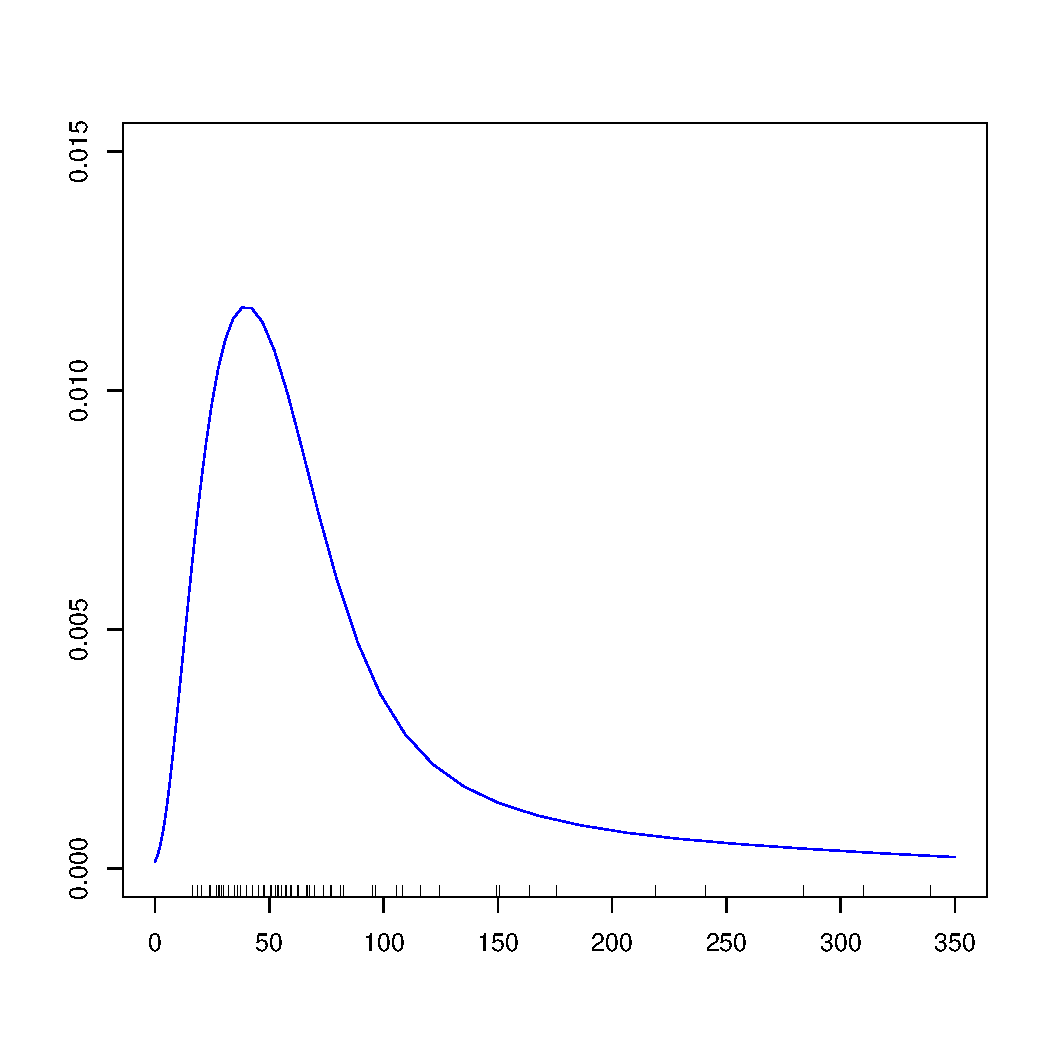
\includegraphics[width=0.7\textwidth]{../common/manual_nt_length_density.pdf}
\caption{A zsoltárok könyve újszövetségi idézettségének szöveghossz-sűrűségbecslése}
\label{kezi-hosszak-suruseg}
\end{center}
\end{figure}

Egy hasonló tesztet végzünk el a Római levél elemzésével. A \ref{tab:Rom-darabszam}. táblázatban
a Római levél 50 olyan szakaszához jegyeztük fel az ószövetségi első egyezést, ahol Pál
konkrétan idézetre utal. Nem számítottuk idézetnek (többek között) a Róma 4:22-t és 4:23-at,
mivel a 4:3-ban már említi Pál apostol az 1Móz 15:6-ot. Nincs a listában a Róma 14:11a
(``Élek én, így szól az Úr'') sem, mivel ez a szófordulat az ÓSZ-ben 17 helyen is megjelenik,
és Pál talán többre vagy akár az \textit{összesre egyszerre} gondol. Hasonlóképpen az olyan utalásokat,
ahol a szövegkörnyezet ezt nem támasztja alá, nem vettük bele a listába, hiába van ezek
között akár egészen hosszú, betű szerint egyező szöveg is (ilyen pl. a Róma 9:20,
ami egész biztosan az Ézs 29:16-ra utal, ez 24 ill. 12 betűnyi teljes egyezést jelentene).

\begin{longtable}{rrrlc}
\caption{A \ref{algo-osz-uszi-ref}. algoritmus által azonosított lehetséges idézetek darabszáma
a tényleges idézeteken belül a Római levélben} \label{tab:Rom-darabszam}\\
{\bf Ssz.}&{\bf Róma-szakasz}&{\bf Hossz}&{\bf ÓSZ-i szakasz}&{\bf Db.}\\
\hline
\endfirsthead
1& 1:17+68 1:17&26&LXX Hab 2:4+39 2:4&1\\
2& 2:24 2:24-14&48&LXX Ézs 52:5+90 52:5&1\\
3& 3:4+63 3:4&56&LXX Zsolt 51:4+43 51:4&2\\
4& 3:11+3 3:18&339&LXX Zsolt 14:2+59 14:3&1\\
5& 4:3+16 4:3&52&LXX 1Móz 15:6+3&1\\
6& 4:7 4:8&92&LXX Zsolt 32:1+15 32:2-30&1\\
7& 4:17+14 4:17-77&29&LXX 1Móz 17:5+57 17:6-67&1\\
8& 4:18+78 4:18&21&LXX 1Móz 15:5+109 15:5&1\\
9& 8:36+14 8:36&62&LXX Zsolt 44:22&1\\
10& 9:7+37 9:7&26&LXX 1Móz 21:12+127 21:12&1\\
11& 9:9+24 9:9&47&LXX 1Móz 18:10+28 18:14&2\\
12& 9:12+39 9:13-43&27&LXX 1Móz 25:23+103 25:24-64&1\\
13& 9:13+29 9:13&31&LXX Mal 1:3 1:3-68&1\\
14& 9:15+16 9:15&37&LXX 2Móz 33:19+87 33:19&1\\
15& 9:17+50 9:17&63&LXX 2Móz 9:16+28 9:16&2\\
16& 9:25+24 9:25-10&37&ABPGRK Hós 2:23+38 2:23-34&0\\
17& 9:26&73&LXX Hós 1:10+82 1:10&1\\
18& 9:27+31 9:27-20&40&LXX Hós 1:10+5 1:10-110&1\\
19& 9:27+46 9:28-15&80&LXX Ézs 10:22+18 10:23-21&2\\
20& 9:29+24 9:29&81&LXX Ézs 1:9+3 1:9&1\\
21& 9:33+14 9:33-5&82&LXX Ézs 28:16+24 28:16&2\\
22& 9:33+30 9:33-54&17&LXX Ézs 8:14+48 8:14-94&0\\
23& 10:5+46 10:5-1&27&LXX 3Móz 18:5+69 18:5-21&1\\
24& 10:6+52 10:8-21&188&LXX 5Móz 30:12+26 30:14-28&1\\
25& 10:13&44&LXX Jóel 2:32+8 2:32-103&1\\
26& 10:15+44 10:15&40&LXX Ézs 52:7 52:7-58&0\\
27& 10:16+45 10:16&28&LXX Ézs 53:1 53:1-31&1\\
28& 10:18+28 10:18&74&LXX Zsolt 19:4 19:4-27&1\\
29& 10:19+41 10:19-40&53&LXX 5Móz 32:21+56 32:21-44&2\\
30& 10:20+24 10:20&60&LXX Ézs 65:1 65:1-42&4\\
31& 10:21+20 10:21&60&LXX Ézs 65:2 65:2-50&2\\
32& 11:3+5 11:3&92&LXX 1Kir 19:10+72 19:10-11&1\\
33& 11:4+27 11:4&62&LXX 1Kir 19:18+3 19:18-30&1\\
34& 11:8+14 11:8&91&LXX 5Móz 29:4+6 29:4-6&2\\
35& 11:8+31 11:8-46&28&LXX Ézs 29:10+22 29:10-61&0\\
36& 11:9+13 11:10&152&LXX Zsolt 69:22 69:23&5\\
37& 11:26+40 11:27-28&73&LXX Ézs 59:20+3 59:21-161&2\\
38& 11:27+28 11:27&28&LXX Ézs 27:9+59 27:9-132&1\\
39& 11:34&45&LXX Ézs 40:13 40:13-14&1\\
40& 12:19+63 12:19-11&22&LXX 5Móz 32:35+7 32:35-73&0\\
41& 12:20+4 12:20&100&LXX Péld 25:21 25:22-28&2\\
42& 13:9+5 13:9-96&32&LXX 2Móz 20:13-15&0\\
43& 13:9+102 13:9&31&LXX 3Móz 19:18+57 19:18-13&1\\
44& 14:11+28 14:11&52&LXX Ézs 45:23+84 45:23&2\\
45& 15:3+46 15:3&42&LXX Zsolt 69:9+34 69:9&1\\
46& 15:9+46 15:9&52&LXX Zsolt 18:49&2\\
47& 15:10+13 15:11-65&30&LXX 5Móz 32:43+60 32:43-172&1\\
48& 15:11+8 15:11&60&LXX Zsolt 117:1+9 117:1&2\\
49& 15:12+19 15:12&64&LXX Ézs 11:10+3 11:10-27&1\\
50& 15:21+17 15:21&58&LXX Ézs 52:15+66 52:15&1\\
\end{longtable}

A táblázat -- mely az újszövetségi idézetek hosszát is megadja --
jól mutatja, hogy a \ref{algo-osz-uszi-ref}. algoritmus az 50-ből mindössze 6
esetben nem tudta beazonosítani a kapcsolatot. Az egyik esetben (a 9:25-nél) ez abból
fakadt, hogy az SBLGNT nem az LXX szövegéhez, hanem az ABPGRK-éhoz hasonlít, de a kereső
szoftver az LXX alapján dolgozott.

A \ref{kezi-hosszak-suruseg-Rom}. ábra az 50 idézet hosszának sűrűségbecslését mutatja.
Ez alapján is látható, hogy Pál apostol nem sajnálja a betűket a pontos szöveg megadására:
a legrövidebb szövege 17 betűs (ez a 9:33-ban megjelenő Ézs 8:14), a következő 21 betűs
(a 4:18-ban hivatkozott 1Móz 15:5), végül egy 22 betűs idézetet is találunk
(a 12:19-ben hivatkozott 5Móz 32:35); a többi hivatkozása azonban legalább 26 betűs. A leghosszabb
egyezés a korábban már említett 339 karakteres szakasz a 14. zsoltárból.

Világos, hogy a \ref{kezi-hosszak-suruseg-Rom}. ábra nem teljesen független
a \ref{kezi-hosszak-suruseg}. ábrától, hiszen a Római levél a Zsoltárokból is idéz.
Szemmel láthatóan azonban a két sűrűségbecslés egymáshoz hasonló jelleget ölt.

\begin{figure}
\begin{center}
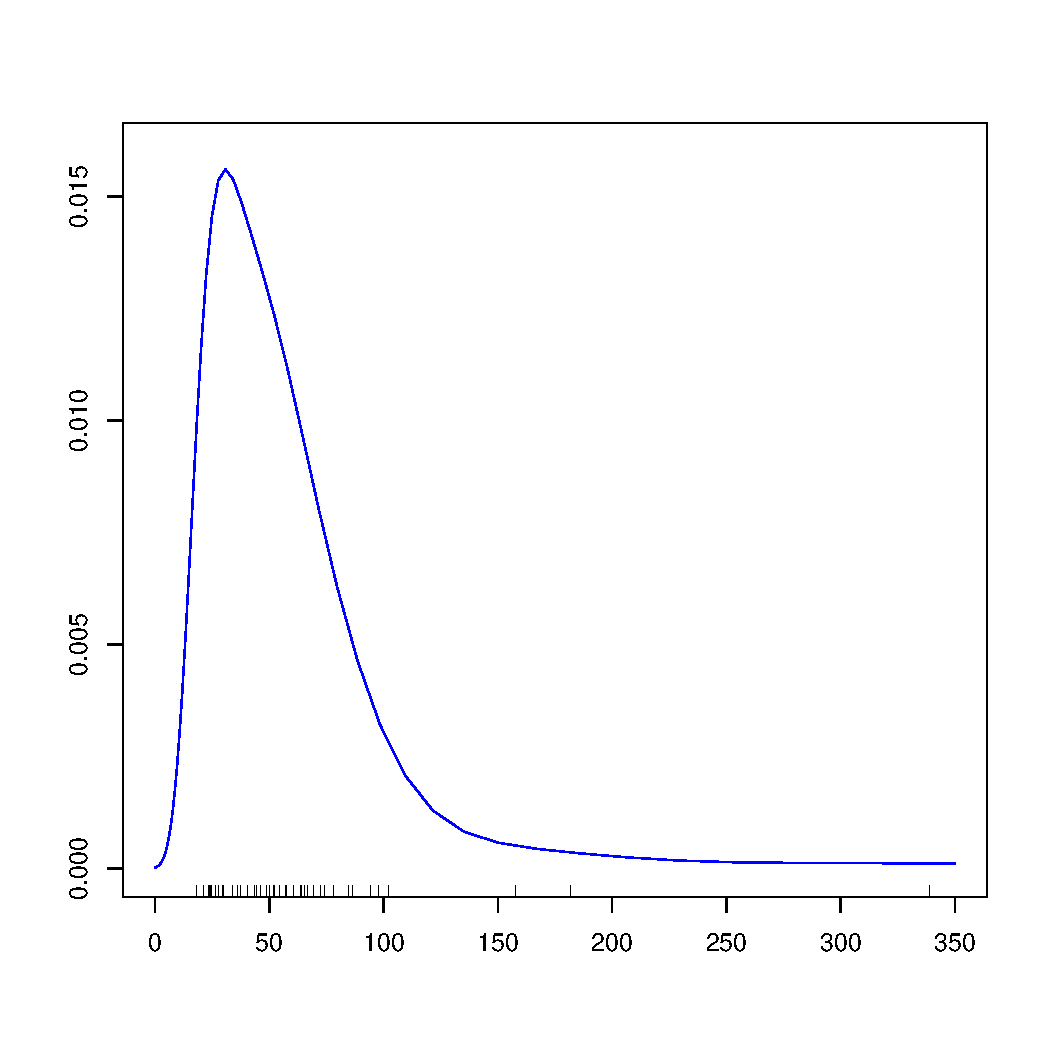
\includegraphics[width=0.7\textwidth]{../common/manual_Romans_length_density.pdf}
\caption{A Római levélben előforduló idézetek szöveghossz-sűrűségbecslése}
\label{kezi-hosszak-suruseg-Rom}
\end{center}
\end{figure}

A Római levél szövege tehát megerősíti, hogy -- bár
a \ref{algo-osz-uszi-ref}. algoritmus majdnem 90\%-os eredményt produkál -- egy fejlettebb
módszerre is szükség van.

Mielőtt továbblépnénk, a Római levél szerkezetét egy további ábrával szemléltetjük.
A \ref{Rom-getrefs}. ábrán szürke pixellel jelöltük a Római levél 34176 karakterének nagy
részét: ezek azok a betűk, amelyek \textit{nem} idézetek. A többi 3014 karakter (ez mintegy
8,82\%) különféle szerepet játszik az idézetek megadásában:

\begin{itemize}
\item Az élénkpiros pixelek a \ref{algo-osz-uszi-ref}. algoritmus által beazonosított
szövegdarabokat jelzik.
\item A sötétpiros pixelek az idézetek további részei, melyeket a \ref{algo-osz-uszi-ref}.
algoritmus nem azonosított be.
\item A fekete pixelek olyan, a \ref{algo-osz-uszi-ref}. algoritmus által detektált
szövegek, melyeket az utólagos kézi ellenőrzés fals pozitív találatnak azonosított.
\item A világoszöld pixelek olyan idézetek, amelyek egy első idézeten belüli
második idézetek, s a \ref{algo-osz-uszi-ref}. algoritmus is megtalálja őket.
\item A sötétzöld pixelek egy első idézeten belüli második idézetek, de csak
a kézi ellenőrzés találta meg őket.
\item A lila színű pixelek nyilvánvalóan idézetek, de esetlegesen több ószövetségi szakaszban
is megtalálhatóak.
\end{itemize}

A pixeleket a bal felső sarokból balról jobbra, majd fentről lefelé kell olvasni. Így pl.
a bal felső pixel a Róma 1:1 első betűjének, míg az utolsó sorokban álló szürke pixelek
a levél utolsó fejezetének felelnek meg. Nagyon intenzív képet kapunk a 9-11. fejezet
környékén: ez a 3 fejezet tartalmazza az idézetek 60\%-át.

\begin{figure}
\begin{center}
\includegraphics[width=\textwidth]{../common/Romans-getrefs}
\caption{Idézetek a Római levélben}
\label{Rom-getrefs}
\end{center}
\end{figure}

\begin{center} *
\end{center}


Plagiátumok keresésekor két szöveg eltérésének mérésére speciális módszerek léteznek.


% A compare12 algoritmus (l. a bibref programot) figyelembe veszi az összehasonlítandó két szöveg
% hosszát: hosszabb szövegeknél, ha az eltérések D száma nő (1-1-gyel), a hossz L is nő (1-1-gyel),
% így általában a D/(L+1) hányados (D+2)/(L+3)-ra változik, ez pedig rendre nagyobb eltérési
% hányadost jelent. (Itt L=L1+L2, ahol L1 és L2 a két szöveg hossza.)
% Habár ez számos esetben hasznos (mivel jelezni akarjuk, hogy az idézett
% szavaknak inkább közel, mintsem távol kell lenniük egymáshoz: vagyis rövid szakaszt tartunk
% inkább idézetnek, mint hosszút, ha nincs teljes egyezésről szó), hosszabb gondolatmeneteknél
% (pl. Pálnál), ahol az egyes idézett szavak egymástól távol is eshetnek, túl nagy eltérést kapunk.
%
% Egy másik lehetőség, hogy nem az eltéréseket, hanem az egyezéseket számoljuk a két szövegben.
% Itt a compare12 által is használt "összes karakterlánc előfordulás" statisztika szerint
% dolgozhatunk. Míg azonban a compare12 2 hosszú karakterláncokról készít statisztikát, itt
% ezt mi 3-ban vagy 4-ben határozzuk meg. (3 hosszúság esetén 25^3=15625, 4 esetén 25^4=390625
% különböző lehetséges karakterlánc van. Ezek kellően egyediek ahhoz, hogy a fals pozitív
% találatok nagy részét kizárjuk.) Az ilyen módon működő statisztikát match12-N algoritmusnak
% nevezzük, ahol N=3 vagy 4. Két szöveg match12-N összehasonlítása tehát úgy történik,
% hogy mindkettőhöz legyártjuk a 25^N db karakterlánchoz tartozó statisztikákat, majd ha
% egy bizonyos ABC karakterlánc az egyik szövegben x-szer, a másikban y-szor jelenik meg, akkor
% a találatok számát min(x,y)-nal növeljük. A találati érték vélhetően kevés lesz, és akkor
% sem nő meg lényegesen, ha a szövegek hosszát valamelyest növeljük.
%
% Az lenne kényelmes, ha a szövegek hosszát egész nagy értékekig növelni lehetne, akár addig
% is, hogy teljes könyveket összehasonlíthassunk. Nagyobb N-re ez jól működhet, úgy viszont
% az N-nél rövidebb szavakat (ill. szókapcsolatokat) nem fogjuk tudni detektálni. Emiatt
% már az N=4 is túl sok lehet.
%
% További probléma, hogy bizonyos karakterláncok gyakoriak a görög nyelvben, és témától
% függetlenül tömegesen előfordulhatnak. Célszerű lehet a szignifikánsan magas gyakoriságú
% karakterláncokat eltávolítani az összes statisztikából.
%
% A fent leírt módon minden egyes bibliai könyvhöz előállíthatunk egy arra jellemző,
% legfeljebb 25^N bejegyzésből álló statisztikát. Ha egy ÓSz-i és egy ÚSz-i könyvet
% ezután a match12-N algoritmussal összehasonlítunk, egy A számot kapunk, mely az
% egyező karakterláncok számát adja (már a szignifikánsan magas gyakoriságúak nélkül).
% Ez az A "szónyi" egyezés leszűkíthető mindkét könyvben egy-egy rövidebb szakaszra.
% Előfordulhat, hogy két igen rövid (egy-két versből álló) szakaszról beszélünk,
% de lehet, hogy jóval hosszabbról. Az első esetben vélhetően megtaláltunk egy
% idézetet (vagy célzást). A második esetben a két szakasz két-két darabra szétvágásával
% (melynek nem feltétlenül kell középen történnie) lehetőségünk nyílik a darabok
% további összehasonlítására. Így pl. a darabok lehetnek Ó1 és Ó2 ill. Ú1 és Ú2,
% s ha match12-N(Ói,Új)+match12-N(Ók,Ól)=A (ahol i,j ill. k,l mind 1 ill. 2 lehetnek),
% akkor a szétvágás során nem vesztünk el egyezést. Ezek után a szűkítést a fentiek
% megismétlésével addig folytatódhat, amíg a rövid egyezéseket mind meg nem találjuk.
%
% Egy teszteset lehet az 1Kor 6:16, ahol 8 karakternyi betoldás van Páltól az
% 1Móz 2:24-t idéző szakaszban.

\textcolor{red}{A szöveg hátralévő része megírásra vár.}

\bibliographystyle{unsrt}
\bibliography{../common/bibref}
\end{document}
